\documentclass[10pt,a4paper]{article}

\usepackage[scaled]{helvet}
\usepackage[left=2.5cm,right=2.5cm,top=3cm,bottom=3cm]{geometry}
\usepackage[none]{hyphenat}\sloppy  % don't hyphenate
\usepackage{tocloft}\addtolength{\cftsubsubsecnumwidth}{0.5em}\tocloftpagestyle{fancy} % fix ToC spacing issue
\usepackage{parskip} % don't indent first line of paragraph
\usepackage{float} % [H]
\usepackage{fancyref} % \Fref
\usepackage{csquotes} % \nquote
\usepackage{enumitem} % [nolistsep]
\usepackage[printonlyused,withpage]{acronym}
\usepackage{tabularx}
\usepackage{makecell}
\usepackage[table]{xcolor}
\usepackage[hidelinks]{hyperref}\hypersetup{colorlinks, allcolors=., urlcolor=teal}
\usepackage[skins]{tcolorbox}
\usepackage{fancyhdr}
\usepackage{titling} % \thetitle, \theauthor
\usepackage{longtable}
\usepackage{array} % \arraybackslash
\usepackage{multicol}
\usepackage{textcomp} % symbols, e.g. \textdegree
\usepackage{textgreek} % greek letters, e.g. \textmu
\usepackage[super]{nth}
\usepackage{sansmath}\sansmath
\usepackage{amsmath} % bmatrix
\usepackage{svg}
\usepackage{macros} % project specific macros

\renewcommand\familydefault{\sfdefault}

\pagestyle{fancy}
\fancyhf{}
\fancyhead[L]{\thetitle{} \version\\ \thedate}
\fancyfoot[R]{\thepage}
\setlength{\headheight}{29pt} % must be large enough for image
\rhead{\includesvg[width=1.5cm]{Images/xioLogo.svg}}
\renewcommand{\headrulewidth}{0.5pt}
\renewcommand{\footrulewidth}{0.5pt}

\renewcommand\labelitemi{\boldmath$\cdot$} % bullet point
\renewcommand\labelitemii{-} % nested bullet point

\author{x-io Technologies}
\title{x-IMU3 User Manual}
\newcommand{\version}{v1.11}
\date{\today}

\begin{document}
    \input{titlePage}

    \clearpage
    \tableofcontents

    \clearpage
    \section{Overview}

\begin{multicols}{2}

The x-IMU3 is x-io Technologies' third generation \ac{IMU}.  It is a high-performance and versatile measurement device designed to accommodate a wide range of data logging and real-time applications including biomechanics, motion-capture, virtual reality, drones, robotics, and industrial.

\acs{USB}, Wi-Fi and Bluetooth provide connectivity for mobile and desktop devices while serial communication supports embedded and industrial systems.  An on-board \acs{microSD} allows the x-IMU3 to function as a stand-alone data logger with the ability to download files by \acs{USB} and Wi-Fi.  Multiple x-IMU3s operating together on the same wireless network will automatically synchronise to stream or log synchronised measurements.

\textbf{Sensors}
\begin{itemize}[nolistsep]
    \item Gyroscope, \textpm{}2000\textdegree{}/s, 400 Hz
    \item Accelerometer, \textpm{}24 g, 400 Hz
    \item Magnetometer, \textpm{}2.5 uT, 20 Hz
    \item High-g accelerometer, \textpm{}200 g, 1600 Hz
    \item Temperature sensor\footnote{The temperature sensor is used for calibration and is not intended to provide an accurate measurement of ambient temperature.}
\end{itemize}

\textbf{Calibration}
\begin{itemize}[nolistsep]
    \item 15-parameter calibration for: axis sensitivity, axis offset, inter-axis misalignment, and package misalignment.
    \item Hard-iron and soft-iron calibration
    \item On-board gyroscope bias correction algorithm
\end{itemize}

\textbf{\acs{AHRS}}
\begin{itemize}[nolistsep]
    \item Algorithm outputs:
    \begin{itemize}
        \item Quaternion
        \item Rotation matrix
        \item Euler angles
        \item Linear acceleration
        \item Earth acceleration
    \end{itemize}
    \item Linear acceleration rejection
    \item Magnetic distortion rejection
    \item 400 Hz update rate
    \item Static accuracy:
        \begin{itemize}
            \item 0.5\textdegree{} \acs{RMS} inclination
            \item 1\textdegree{} \acs{RMS} heading
        \end{itemize}
\end{itemize}

\columnbreak

\textbf{Communication}
\begin{itemize}[nolistsep]
    \item \acs{USB} (\acs{CDC})
    \item Serial, 3.3V \acs{UART}
    \item \acs{TCP} (Wi-Fi)
    \item \acs{UDP} (Wi-Fi)
    \item Bluetooth\footnote{Bluetooth connectivity is currently in development and not yet supported.}
\end{itemize}

\textbf{Wi-Fi}
\begin{itemize}[nolistsep]
    \item Client and \acs{AP} mode
    \item Dual band (2.4 GHz, 5 GHz)
    \item WPA/WPA2-Personal
    \item WPA/WPA2-Enterprise\footnote{WPA/WPA2-Enterprise security is currently in development and not yet supported. Will only be supported in client mode.}
\end{itemize}

\textbf{Data logging}
\begin{itemize}[nolistsep]
    \item Supports \acsp{microSD} up to 32 GB\footnote{The product is supplied with an 8 GB \acs{microSD} that can be upgraded by the user.}
    \item Start/stop logging remotely
    \item USB download
    \item Wi-Fi download\footnote{Wi-Fi downloading is currently in development and not yet supported.}
    \item \acs{CSV} output
\end{itemize}

\textbf{Serial accessories}
\begin{itemize}[nolistsep]
    \item Receive data from external sensors and user electronics, e.g. \acs{GPS}, analogue/digital inputs, application-specific sensors.
    \item 3.3 V output to power external electronics
\end{itemize}

\textbf{Battery}
\begin{itemize}[nolistsep]
    \item Internal battery charged by \acs{USB}
    \item 20 hours data logging
    \item 15 hours Bluetooth
    \item 12 hours Wi-Fi client 2.4 GHz
    \item 8 hours Wi-Fi client 5 GHz
\end{itemize}

\textbf{Housing}
\begin{itemize}[nolistsep]
    \item \acs{IP67}
    \item Wearable strap or chassis mount
\end{itemize}

\textbf{Software \acs{GUI}}
\begin{itemize}[nolistsep]
    \item Connect to multiple x-IMU3s
    \item Real-time data graphs and 3D view
    \item Log data to \acs{CSV}
    \item Windows, macOS, Ubuntu
\end{itemize}

\textbf{Software \acs{API}}
\begin{itemize}[nolistsep]
    \item Rust, C, C++, C\#, Python
    \item Code examples for other languages available
\end{itemize}

\end{multicols}

\clearpage

    \section{Hardware}

\subsection{Board}

Board components are annotated in \Fref{fig:board}.  A detailed mechanical drawing describing the board dimensions and locations of key components is available on the \productWebPage{}.

\vskip 2em

\begin{figure}[H]
    \centering
    \begin{tikzpicture}[annotation/.style={circle, draw=black, fill=white, very thick, minimum size=7mm}]
        \node at (0,0) {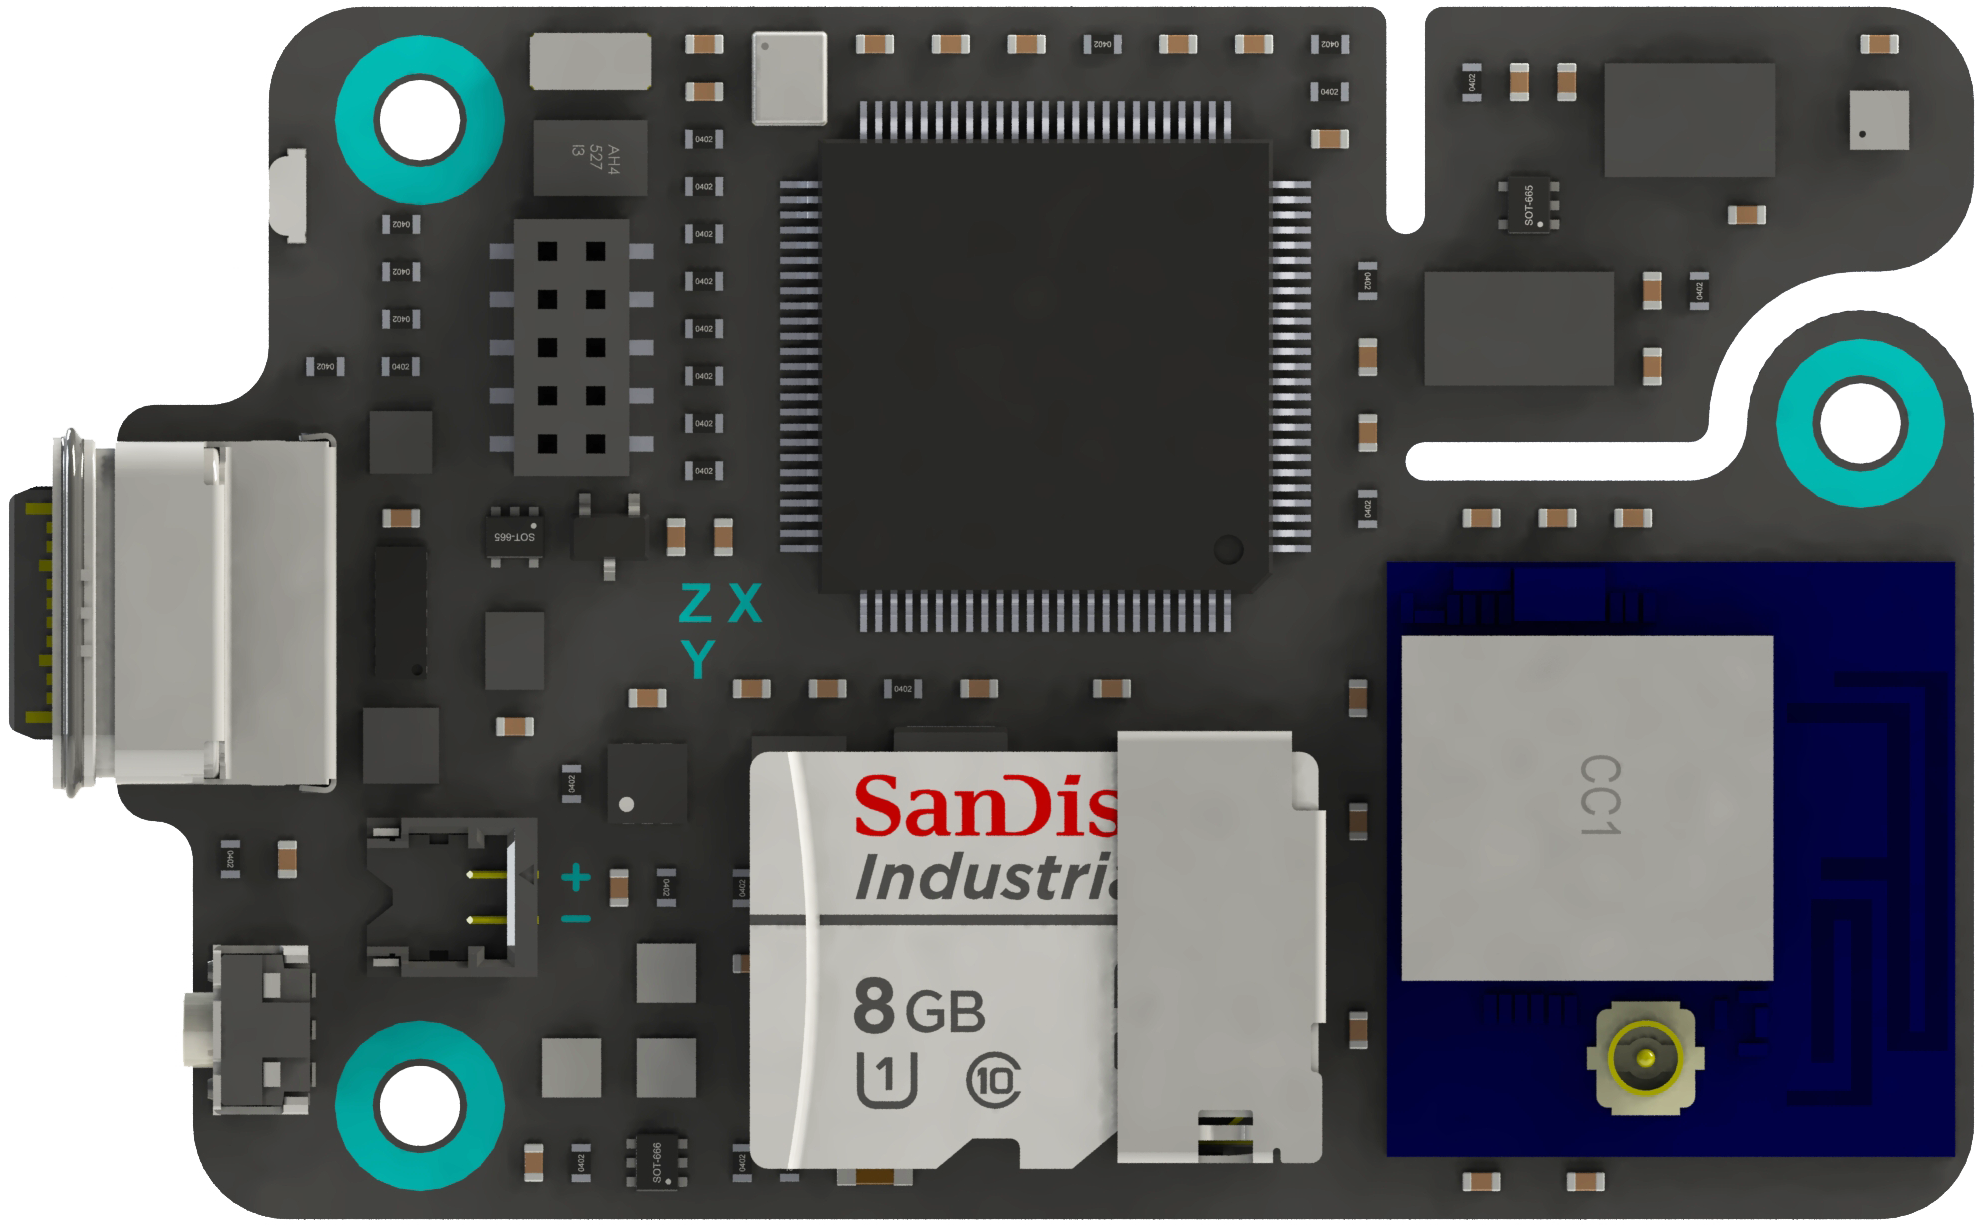
\includegraphics[width=0.95\textwidth]{Images/board.png}};
        \node[annotation] at (-6,-4) {\ref{itm:board1}};
        \node[annotation] at (-6.4,0) {\ref{itm:board2}};
        \node[annotation] at (-5.7,3.7) {\ref{itm:board3}};
        \node[annotation] at (-2.7,1.1) {\ref{itm:board4}};
        \node[annotation] at (4.8,1.8) {\ref{itm:board5}};
        \node[annotation] at (6.0,3.4) {\ref{itm:board6}};
        \node[annotation] at (7.2,3.4) {\ref{itm:board7}};
        \node[annotation] at (6.8,-1.9) {\ref{itm:board8}};
        \node[annotation] at (5.5,-4) {\ref{itm:board9}};
        \node[annotation] at (1.7,-2.5) {\ref{itm:board10}};
        \node[annotation] at (-3.4,-2.9) {\ref{itm:board11}};
    \end{tikzpicture}
    \caption{Board}
    \label{fig:board}
\end{figure}

\vskip 1em

\begin{enumerate}
    \item \label{itm:board1} Power button
    \item \label{itm:board2} \acs{USB}-C connector
    \item \label{itm:board3} \acs{LED}
    \item \label{itm:board4} Serial header
    \item \label{itm:board5} High-g accelerometer
    \item \label{itm:board6} Inertial sensor (gyroscope and accelerometer)
    \item \label{itm:board7} Magnetometer
    \item \label{itm:board8} Wireless antennae
    \item \label{itm:board9} U.FL connector for external wireless antennae
    \item \label{itm:board10} \acs{microSD} socket
    \item \label{itm:board11} Battery connector
\end{enumerate}

\clearpage

\subsubsection{Serial header}

\newcommand{\partNumber}[1] {\enquote{\href{https://www.samtec.com/products/#1}{#1}}}

The serial header pinout is annotated in \fref{fig:serialHeaderPinout}.  The connector part number is \partNumber{CLP-105-02-L-D}.  The recommend mating connector part number is \partNumber{FTS-105-03-F-DV}.

% import numpy

% width = 1.3
% height = 1.5
% pin = 1

% for y in numpy.linspace(height, -height, 5):
%     for x in numpy.linspace(-width, width, 2):
%         print("        \\node[annotation] at (" + "{:.2f}".format(x) + "," + "{:.2f}".format(y) + ") {" + str(pin) + "};")
%         pin += 1

\begin{figure}[H]
    \centering
    \begin{tikzpicture}[annotation/.style={draw=black, fill=white, very thick, minimum size=6mm}]
        \node at (0,0) {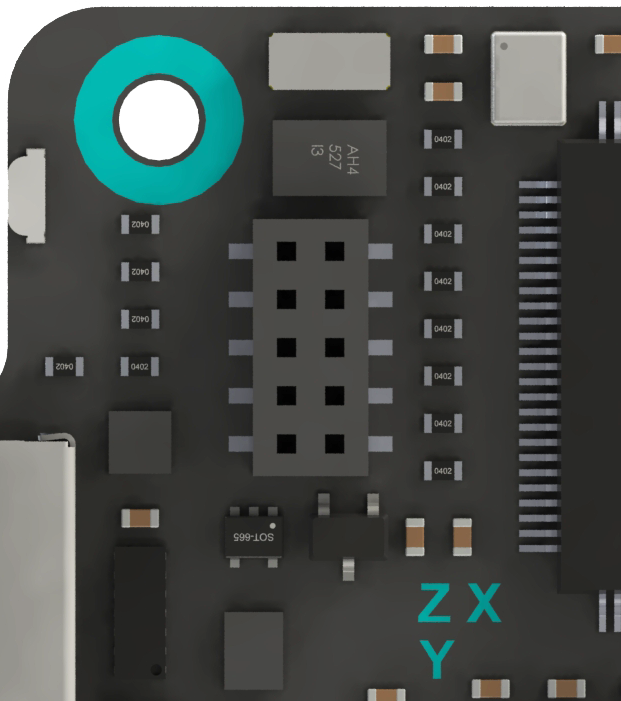
\includegraphics[width=0.5\textwidth]{Images/serialHeader.png}};
        \node[annotation] at (-1.30,1.50) {1};
        \node[annotation] at (-1.30,0.75) {2};
        \node[annotation] at (-1.30,0.00) {3};
        \node[annotation] at (-1.30,-0.75) {4};
        \node[annotation] at (-1.30,-1.50) {5};
        \node[annotation] at (1.30,1.50) {6};
        \node[annotation] at (1.30,0.75) {7};
        \node[annotation] at (1.30,0.00) {8};
        \node[annotation] at (1.30,-0.75) {9};
        \node[annotation] at (1.30,-1.50) {10};
    \end{tikzpicture}
    \caption{Serial header pinout}
    \label{fig:serialHeaderPinout}
\end{figure}

\customTable
{l l l}
{Pin & Name & Type}
{
    1 & 3.3V & Power\\
    2 & GND  & Power\\
    3 & VBAT  & Power\\
    4 & VBUS  & Power\\
    5 & Button  & Input\\
    6 & Serial override & Input\\
    7 & Serial \ac{RTS} & Output\\
    8 & Serial \ac{CTS} & Input\\
    9 & Serial \ac{RX} & Input\\
    10 & Serial \ac{TX} & Output\\
}
{Serial header pinout}
{tab:serialHeaderPinout}

\vskip 1em

\warning{Incorrect connections to the serial header may cause permanent damage.  This interface should only be used by an experienced engineer.}

\clearpage

\subsection{Housing}

The housing interfaces are annotated in \Fref{fig:housing}.  A detailed mechanical drawing describing the housing dimensions is available on the \productWebPage{}.

\vskip 2em

\begin{figure}[H]
    \centering
    \begin{tikzpicture}[annotation/.style={circle, draw=black, fill=white, very thick, minimum size=7mm}]
        \node at (0,0) {\includegraphics[width=0.8\textwidth]{Images/housing.png}};
        \node[annotation] at (-5.6,-2) {\ref{itm:housing1}};
        \node[annotation] at (-3.7,-2.55) {\ref{itm:housing2}};
        \node[annotation] at (-1.2,-3.2) {\ref{itm:housing3}};
    \end{tikzpicture}
    \caption{Housing}
    \label{fig:housing}
\end{figure}

\vskip 1em

\begin{enumerate}
    \item \label{itm:housing1} Power button
    \item \label{itm:housing2} \acs{USB}-C connector
    \item \label{itm:housing3} \acs{LED}
\end{enumerate}

\subsubsection{\acs{IP67} rating}

The \ac{IP67} rating is an international standard that describes the ability of the housing to protect against the ingress of solid particles and water.  The first digit, 6 indicates complete protection against dust and solid particles.  The second digit, 7 indicates protection from water for a maximum depth of 1 meter for up to 30 minutes.

In practical terms, this means that the housing can be used outdoors in all weather conditions and that it will survive accidental or temporary submersion in water.  The housing should \underline{not} be used in underwater applications.

\clearpage

    \section{Technical specification}

\newcommand{\techincalTable}[5]{
    \customTable
    {l c c}
    {#1 & Value & Notes}
    {
        #2
    }
    {#3}
    {#4}
    \textbf{Notes}
    \begin{enumerate}[nolistsep]
        #5
    \end{enumerate}
}

\newcommand{\characteristicTable}[4]{
    \techincalTable
    {Characteristic}
    {#1}
    {#2}
    {#3}
    {#4}
}

\newcommand{\conditionTable}[4]{
    \techincalTable
    {Condition}
    {#1}
    {#2}
    {#3}
    {#4}
}

\subsection{Mechanical}

\subsubsection{Board}

\newcommand{\noteMechanicalDrawings}[1]{A detailed mechanical drawing describing the #1 dimensions and locations of key components is available on the \productWebPage{}.}

\characteristicTable
{
    Size & 52 $\times$ 32 $\times$ 5 mm & \ref{itm:boardMechanicalSpecification1}\\
    Weight & 8 g & -\\
}
{Board mechanical specification}
{tab:boardMechanicalSpecification}
{
    \item \label{itm:boardMechanicalSpecification1} \noteMechanicalDrawings{board}
}

\subsubsection{Housing}

\characteristicTable
{
    Size & 55 $\times$ 50 $\times$ 14 mm & \ref{itm:housingMechanicalSpecification1}\\
    Weight & 31 g & -\\
}
{Housing mechanical specification}
{tab:housingMechanicalSpecification}
{
    \item \label{itm:housingMechanicalSpecification1} \noteMechanicalDrawings{housing}
}

\subsection{Temperature}
\label{sec:temperature}

\newcommand{\noteHeat}{The operating temperature of the device will always be greater than the surroundings due to heat generated by electronics.}

\newcommand{\noteFullRange}{The specified accuracy of the device is not achieved over the full operating temperature range.  \seeSection{sec:calibration}}

\subsubsection{No battery}

\characteristicTable
{
    Operating & -40\textdegree{}C to 85\textdegree{}C & \ref{itm:temperatureNoBattery1}, \ref{itm:temperatureNoBattery2}\\
    Storage & -40\textdegree{}C to 105\textdegree{}C & -\\
}
{Temperature specification (no battery)}
{tab:temperatureSpecificationNoBattery}
{
    \item \label{itm:temperatureNoBattery1} \noteHeat
    \item \label{itm:temperatureNoBattery2} \noteFullRange
}

\subsubsection{With battery}

\characteristicTable
{
    Operating (discharging) & -20\textdegree{}C to 60\textdegree{}C & \ref{itm:temperatureWithBattery1}, \ref{itm:temperatureWithBattery2}\\
    Operating (charging) & 0\textdegree{}C to 45\textdegree{}C & \ref{itm:temperatureWithBattery1}, \ref{itm:temperatureWithBattery2}, \ref{itm:temperatureWithBattery3}\\
    Storage & -20\textdegree{}C to 25\textdegree{}C & -\\
}
{Temperature specification (with battery)}
{tab:temperatureSpecificationWithBattery}
{
    \item \label{itm:temperatureWithBattery1} \noteHeat
    \item \label{itm:temperatureWithBattery2} \noteFullRange
    \item \label{itm:temperatureWithBattery3} Charging at temperatures below 0\textdegree{}C will reduce the capacity and cycle life of the battery.
}

\subsection{Sensors}

\newcommand{\noteRate}[1]{Each #1 includes a timestamp for a reliable measurement of time independent of the #1 rate error.  \seeSection{sec:sampleRatesMessageRatesAndTimestamps}}

\newcommand{\noteBandwidth}{The maximum bandwidth is achieved when the message rate is equal to the sample rate.  If the message rate is less than the sample rate then samples are averaged.  \seeSection{sec:sampleRatesMessageRatesAndTimestamps}}

\newcommand{\noteAccuracy}[3]{The #1 error is evaluated as the deviation of the measured magnitude of #2 for a 360\textdegree{} rotation around each axis aligned to the #3.  The magnitude is calculated as $\sqrt{x^2 + y^2 + z^2}$.}

\newcommand{\noteTemperature}{Accuracy is specified for the calibrated temperature only. \seeSection{sec:calibration}}

\subsubsection{Gyroscope}

\characteristicTable
{
    Range & \textpm{}2000\textdegree{}/s & -\\
    Resolution & 16-bit, 0.061\textdegree{}/s & -\\
    Sample rate & 400 Hz \textpm{}0.3\% & \ref{itm:gyroscope1}\\
    Bandwidth & 47 Hz & \ref{itm:gyroscope2}\\
    Noise & 0.014\textdegree{}/s/$\surd$Hz & -\\
}
{Gyroscope specification}
{tab:gyroscopeSpecification}
{
    \item \label{itm:gyroscope1} \noteRate{sample}
    \item \label{itm:gyroscope2} \noteBandwidth
}

\subsubsection{Accelerometer}

\characteristicTable
{
    Range & \textpm{}24 g & -\\
    Resolution & 16-bit, 732 \textmugreek{}g & -\\
    Sample rate & 400 Hz \textpm{}0.3\% & \ref{itm:accelerometer1}\\
    Bandwidth & 145 Hz & \ref{itm:accelerometer2}\\
    Noise & 160 \textmugreek{}g/$\surd$Hz (X, Y), 190 \textmugreek{}g/$\surd$Hz (Z) & -\\
    Accuracy at 1 g & \textpm{}5 mg & \ref{itm:accelerometer3}, \ref{itm:accelerometer4}\\
}
{Accelerometer specification}
{tab:accelerometerSpecification}
{
    \item \label{itm:accelerometer1} \noteRate{sample}
    \item \label{itm:accelerometer2} \noteBandwidth
    \item \label{itm:accelerometer3} \noteAccuracy{accelerometer}{gravity}{horizontal}
    \item \label{itm:accelerometer4} \noteTemperature
}

\subsubsection{Magnetometer}

\characteristicTable
{
    Range & \textpm{}1300 \textmugreek{}T (X, Y), \textpm{}2500 \textmugreek{}T (Z) & -\\
    Sample rate & 20 Hz \textpm{}8\% & \ref{itm:magnetometer1}\\
    Noise & 0.3 \textmugreek{}T & -\\
    Accuracy at 1 \acs{a.u.} & \textpm{}50 m\acs{a.u.} & \ref{itm:magnetometer2}, \ref{itm:magnetometer3}, \ref{itm:magnetometer4}\\
}
{Magnetometer specification}
{tab:magnetometerSpecification}
{
    \item \label{itm:magnetometer1} \noteRate{sample}
    \item \label{itm:magnetometer2} The calibrated magnetometer units are \ac{a.u.}.  1 \ac{a.u.} is equal to the magnitude of the ambient magnetic field during calibration, approximately 50 \textmugreek{}T.
    \item \label{itm:magnetometer3} \noteAccuracy{magnetometer}{the ambient magnetic field}{vertical}
    \item \label{itm:magnetometer4} \noteTemperature
}

\subsubsection{High-g accelerometer}

\characteristicTable
{
    Range & \textpm{}200 g & -\\
    Resolution & 16-bit, 6.1 mg & -\\
    Sample rate & 1600 Hz \textpm{}2\% & \ref{itm:highGAccelerometer1}\\
    Bandwidth & 800 Hz & \ref{itm:highGAccelerometer2}\\
    Noise & 5 mg/$\surd$Hz & -\\
    Accuracy at 1 g & \textpm{}150 mg & \ref{itm:highGAccelerometer3}, \ref{itm:highGAccelerometer4}\\
}
{High-g accelerometer specification}
{tab:highGAccelerometerSpecification}
{
    \item \label{itm:highGAccelerometer1} \noteRate{sample}
    \item \label{itm:highGAccelerometer2} \noteBandwidth
    \item \label{itm:highGAccelerometer3} \noteAccuracy{accelerometer}{gravity}{horizontal}
    \item \label{itm:highGAccelerometer4} \noteTemperature
}

\subsubsection{Temperature sensor}

\characteristicTable
{
    Range & -104\textdegree{}C to 150\textdegree{}C & \ref{itm:temperatureSensor1}\\
    Sample rate & 5 Hz \textpm{}0.3\% & \ref{itm:temperatureSensor2}, \ref{itm:temperatureSensor3}\\
    Accuracy & \textpm{}1\textdegree{}C at 25\textdegree{}C & -\\
}
{Temperature sensor specification}
{tab:temperatureSensor}
{
    \item \label{itm:temperatureSensor1} The temperature sensor measurement range exceeds the device operating temperature range.  \seeSection{sec:temperature}
    \item \label{itm:temperatureSensor2} \noteRate{sample}
    \item \label{itm:temperatureSensor3} The temperature sensor is oversampled and the result decimated to the specified sample rate.
}

\subsection{\acs{AHRS}}

\subsubsection{Update rate}

\characteristicTable
{
    Update rate & 400 Hz \textpm{}0.3\% & \ref{itm:ahrsUpdateRate1}, \ref{itm:ahrsUpdateRate2}\\
}
{\acs{AHRS} update rate}
{tab:ahrsUpdateRate}
{
    \item \label{itm:ahrsUpdateRate1} \noteRate{update}
    \item \label{itm:ahrsUpdateRate2} The \ac{AHRS} update rate is fixed independent of message rate settings.  \ac{AHRS} outputs are not averaged when the message rate is less than the update rate.
}

\subsubsection{Static accuracy}

\characteristicTable
{
    Inclination & 0.5\textdegree{} \acs{RMS} & \ref{itm:ahrsStaticAccuracy1}, \ref{itm:ahrsStaticAccuracy2}\\
    Heading & 1\textdegree{} \acs{RMS} & \ref{itm:ahrsStaticAccuracy1}, \ref{itm:ahrsStaticAccuracy2}\\
}
{\acs{AHRS} static accuracy}
{tab:ahrsStaticAccuracy}
{
    \item \label{itm:ahrsStaticAccuracy1} Static accuracy is specified as the \ac{RMS} error for a 360\textdegree{} rotation around each axis.
    \item \label{itm:ahrsStaticAccuracy2} \noteTemperature
}

\subsection{Data logger capacity}

\newcommand{\noteBinary}{The data logging capacity is specified for binary data messages.  Capacity will be reduced for \acs{ASCII} data messages.}

\subsubsection{8 GB \acs{microSD}}

\conditionTable
{
    Default message rates & 485 hours & \ref{itm:dataLoggerCapacity8GB1}\\
    Maximum message rates & 23 hours & \ref{itm:dataLoggerCapacity8GB1}\\
}
{Data logger capacity for 8 GB \acs{microSD}}
{tab:dataLoggerCapacity8GB1}
{
    \item \label{itm:dataLoggerCapacity8GB1} \noteBinary
}

\subsubsection{32 GB \acs{microSD}}

\conditionTable
{
    Default message rates & 1941 hours & \ref{itm:dataLoggerCapacity32GB1}, \ref{itm:dataLoggerCapacity32GB2}\\
    Maximum message rates & 94 hours & \ref{itm:dataLoggerCapacity32GB1}, \ref{itm:dataLoggerCapacity32GB2}\\
}
{Data logger capacity for 32 GB \acs{microSD}}
{tab:dataLoggerCapacity32GB1}
{
    \item \label{itm:dataLoggerCapacity32GB1} \noteBinary
    \item \label{itm:dataLoggerCapacity32GB2} The product is supplied with an 8 GB \acs{microSD} that can be upgraded by the user.  The maximum compatible \acs{microSD} capacity is 32 GB.
}

    \input{Sections/calibration}
    \input{Sections/powerButton}
    \section{\acs{LED}}
\label{sec:led}

The \ac{LED} indicates the mode and status of the x-IMU3 using different colours and flashing behaviours.

\newcommand{\ledFigure}[2]{
    \begin{figure}[H]
        \centering
        \includegraphics[width=0.5\textwidth]{Images/#1.png}
        \caption{#2}
        \label{fig:#1}
    \end{figure}
}

\subsection{Wireless disabled (green)}

A green \ac{LED}, as shown in \Fref{fig:greenLed} indicates that the x-IMU3 is switched on and that the wireless mode is disabled.  In this mode, the \ac{LED} indicates the data logger state.  Flashing indicates that the data logger is disabled and a solid \ac{LED} indicates that the data logger is enabled.

\ledFigure{greenLed}{Green \acs{LED} indicating that the x-IMU3 is switched on and that the wireless mode is disabled}

\subsection{Wi-Fi client (cyan)}

A cyan \ac{LED}, as shown in \Fref{fig:cyanLed} indicates that the x-IMU3 is switched on and in Wi-Fi client mode. Slow flashing (once per second) indicates that x-IMU3 is not connected to an \ac{AP}, fast flashing (five times per second) indicates that the x-IMU3 is connected to an \ac{AP} but has not yet obtained an \ac{IP} address, and a solid \ac{LED} indicates that the x-IMU3 is connected to an \ac{AP} and has an \ac{IP} address.

\ledFigure{cyanLed}{Cyan \acs{LED} indicating that the x-IMU3 is switched on and in Wi-Fi client mode}

\subsection{Wi-Fi AP (magenta)}

A magenta \ac{LED}, as shown in \Fref{fig:magentaLed} indicates that the x-IMU3 is switched on and in Wi-Fi \ac{AP} mode.  The \ac{LED} will flash during the initialisation of the Wi-Fi network.  Once the network has been created, the \ac{LED} will remain solid.

\ledFigure{magentaLed}{Magenta \acs{LED} indicating that the x-IMU3 is switched on and in Wi-Fi \acs{AP} mode}

\subsection{Bluetooth (blue)}

A blue \ac{LED}, as shown in \Fref{fig:blueLed} indicates that the x-IMU3 is switched on and in Bluetooth mode.  Slow flashing (once per second) indicates that Bluetooth is not connected and the x-IMU3 is not discoverable, fast flashing (five times per second) indicates that Bluetooth is not connected and the x-IMU3 is discoverable, and a solid \ac{LED} indicates that Bluetooth is connected.  The x-IMU3 is not discoverable while Bluetooth is connected.

\ledFigure{blueLed}{Blue \acs{LED} indicating that the x-IMU3 is switched on and in Bluetooth mode}

\subsection{Error (red)}

A red \ac{LED}, as shown in \Fref{fig:redLed} indicates an error.  The \ac{LED} will interrupt it's normal behaviour to blink red each time an error message is sent by the x-IMU3.

\ledFigure{redLed}{Red \acs{LED} indicating an error}

\subsection{Low battery and charging (orange)}

An orange \ac{LED}, as shown in \Fref{fig:orangeLed} indicates either a low battery the x-IMU3 is switched on, or the charging status if the x-IMU3 is switched off.  The \ac{LED} will interrupt it's normal behaviour to blink orange once a second to indicate that the battery is low.  If the x-IMU3 is switched off and USB power is connected then the \ac{LED} will remain solid while the x-IMU3 is charging and blink once every four seconds once charging is complete.

\ledFigure{orangeLed}{Orange \acs{LED} indicating low battery or charging status}

\subsection{User control}

The \ac{LED} can be controlled by the user using the strobe and colour commands.  See \Fref{sec:strobeCommand} and \Fref{sec:colourCommand} for more information.

     \section{Wi-Fi}

\subsection{Mode}

\subsubsection{Client}

...

\subsubsection{\acs{AP}}

This is a use of the acronym \ac{AP}.

\subsection{\acs{TCP}}

This is a use of the acronym \ac{TCP}.

\subsection{\acs{UDP}}

This is a use of the acronym \ac{UDP}.

\subsection{Network configurations}

...

\subsubsection{\acs{AP} mode for single device}

...

\subsubsection{\acs{AP} mode for multiple devices}

...

\subsubsection{Hotspot}

...

\subsubsection{Router with \acs{LAN} connection}

This is a use of the acronym \ac{LAN}.

\subsubsection{Router with Wi-Fi connection}

...

    \section{Data logger}
\label{sec:dataLogger}

The x-IMU3 can function as a stand-alone data logger by streaming real-time data to a file on the \ac{microSD}.  Files created by the data logger use the .ximu3 extension and can be downloaded from the x-IMU3 to be converted to \ac{CSV} files using the product software.

The data logger will create a new file in the \enquote{Data Logger} directory on the \ac{microSD} each time logging starts.  Files will never be overwritten or deleted by the data logger.  If the \ac{microSD} becomes full then the data logger will stop and the x-IMU3 will indicate an error.

\subsection{Start and stop}

The data logger is enabled or disabled in the device settings.  If the data logger is enabled then logging will start when the x-IMU3 is switched on and stop when the x-IMU3 is switched off.  Alternatively, an application can start and stop logging remotely by enabling and disabling the data logger while the x-IMU3 is switched on.

\subsection{File name}
\label{sec:fileName}

The file name format is \enquote{prefix\_YYYY-MM-DD\_hh-mm-ss\_CCCC.ximu3} where where "prefix" is a user-defined label configured in the device settings, \enquote{YYYY-MM-DD\_hh-mm-ss} is the time that the file was created, and \enquote{CCCC} is a counter.  If the prefix is left blank then the device serial number will be used with the format \enquote{XXXXXXXX}.  The time and counter parts of the file name can be individually enabled or disabled in the device settings.  For example, if the counter was disabled and the prefix left blank for an x-IMU3 with the serial number \enquote{01234567} then a file created at 3.30 p.m. on January 20, 2025 would have the name \enquote{01234567\_2025-01-20\_15-30-00.ximu3}.

The counter is a four digit number between 0000 and 9999 that increments each time it is used.  If a file name using the counter already exists then the counter will increment until the file name is available.  Incrementing beyond 9999 will cause the counter to wraparound to 0000.  If the counter part of the file name is disabled and the file name already exists then the counter will used automatically to create an available file name.

\subsection{File contents}

The contents of the file is a byte stream as per the communication protocol described in \Fref{sec:communicationProtocol}.  Each file starts with a preamble of the following messages, in order.

\begin{enumerate}[nolistsep]
    \item Ping response
    \item Write time command
    \item Write setting command for each setting
\end{enumerate}

\subsection{Maximum file size and period}
\label{sec:maximumFileSizeAndPeriod}

A maximum file size and maximum file period can be configured in the device settings.  The data logger will start a new file each time the file size reaches the maximum file size, or the period since the start of the file reaches the maximum file period.

\subsection{Downloading files}

Data logger files can be download by \ac{USB} or Wi-Fi.  The \ac{microSD} appears as an external drive when \ac{USB} is connected.  The \ac{microSD} cannot be accessed while the data logger is enabled.  The contents of the \enquote{Data Logger} directory on the \ac{microSD} can be accessed by Wi-Fi by typing in the x-IMU3's \ac{IP} address to a browser.  This directory cannot be accessed while the data logger is enabled.

    \section{Communication protocol}
\label{sec:communicationProtocol}

All communication interfaces use the same communication protocol.  The byte stream is therefore identical for \ac{USB}, serial, \ac{TCP}, \ac{UDP}, Bluetooth, and the files created by the data logger.  The communication protocol consists of two message types:

\begin{itemize}[nolistsep]
    \item Command messages
    \item Data messages
\end{itemize}

All messages are terminated by a \ac{LF} control character.  This termination byte will not appear anywhere else in a message and so can be used to divide a byte stream into individual messages.  \Fref{tab:controlCharactersLFrepresentations} describes the different ways that the control character \ac{LF} may be referred to throughout this document.

\customTable
{l c c c c}
{Control character & Abbreviation & String & Hex & Decimal}
{
    \acl{LF} & \acs{LF} & \enquote{\textbackslash n} & 0x0A & 10\\
}
{Control characters \acs{LF} representations}
{tab:controlCharactersLFrepresentations}

The first byte of a message indicates the message type.  Command messages start with the character \enquote{\{} (0x7B in hex, 123 in decimal).  Data messages start with either an uppercase character or a byte value greater than 0x80 (128 in decimal) depending on the message.

\subsection{Command messages}

Command messages are sent to the x-IMU3 to read and write settings and execute commands.  All command messages are a \ac{JSON} object containing a single key/value pair, terminated by the control character \ac{LF}.  The control character \ac{LF} must not appear anywhere else in a command message.  The x-IMU3 will acknowledge each received command message by sending a command message with the same key to the host.

The key used by command messages sent to the x-IMU3 is not case sensitive and can use non-alphanumeric characters arbitrarily.  For example, \enquote{serialNumber}, \enquote{Serial Number}, and \enquote{serial\_number} are all valid keys for a command message to read the device serial number.

\newcommand{\commandMessageExample}[2]{
    \begin{table}[H]
        \def\arraystretch{1.5}
        \begin{tabular}{l l}
            \textbf{Example:} & \texttt{\{#1\}\textbackslash n}
        \end{tabular}
    \end{table}
}

\subsubsection{Read setting command}

The read setting command is sent to the x-IMU3 to read a setting value.  The key is the setting key and the value is null.  See \Fref{sec:individualSettings} for a complete list of settings.  The x-IMU3 will acknowledge a read setting command by sending a write setting command to the host.

\commandMessageExample{"serialNumber":null}

\subsubsection{Write setting command}

The write setting command is sent to the x-IMU3 to write a setting value, or sent from the x-IMU3 to the host in response to a read setting command.  The key is the setting key and the value is the setting value.  See \Fref{sec:individualSettings} for a complete list of settings.  The x-IMU3 will acknowledge a write setting command by sending a setting write command back to the host, indicating the new settings value.  The x-IMU3 will not apply new settings until two seconds after the most recent write setting command or default command was received.

\commandMessageExample{"deviceName":"x-IMU3"}

\subsubsection{Default command}

The default command is sent to the x-IMU3 to set all settings to default values.  The key is \enquote{default} and the value is null.  The x-IMU3 will not apply new settings until two seconds after the most recent write setting command or default command was received.

\commandMessageExample{"default":null}

\subsubsection{Apply command}

The apply command is sent to the x-IMU3 to apply all settings.  The key is \enquote{apply} and the value is null.  This command can be sent after a write setting or default command to apply settings immediately instead of after a two second delay.

\commandMessageExample{"apply":null}

\subsubsection{Save command}

The save command is sent to the x-IMU3 to save all settings to \ac{EEPROM}.  The key is \enquote{save} and the value is null.  The command acknowledgement will not be sent until the save is complete.  This may take up to 300 milliseconds.  The save command is unnecessary in most applications because the x-IMU3 will automatically save all settings on shutdown.

\commandMessageExample{"save":null}

\subsubsection{Read time command}

The read time command is sent to the x-IMU3 to read the date and time of the \ac{RTC}.  The key is \enquote{time} and the value is null.  The x-IMU3 will acknowledge a read time command by sending a write time command to the host.

\commandMessageExample{"time":null}

\subsubsection{Write time command}

The write time command is sent to the x-IMU3 to write the date and time of the \ac{RTC}, or sent from the x-IMU3 to the host in response to a read time command.  The key is \enquote{time} and the value is a string expressing the date and time in the format \enquote{YYYY-MM-DD hh:mm:ss} where each delimiter can be any non-numerical character.  The x-IMU3 will acknowledge a write time command by sending a write time command back to the host, indicating the new date and time.

\commandMessageExample{"time":"2020-01-01 00:00:00"}

\subsubsection{Ping command}

The ping command is sent to the x-IMU3 to trigger a ping response.  The key is \enquote{ping} and the value is null.  The x-IMU3 will acknowledge a ping command by sending a ping response to the host.

\commandMessageExample{"ping":null}

\subsubsection{Ping response}

The ping response is sent from the x-IMU3 to the host in response to the ping command.  The key is \enquote{ping} and the value is a \ac{JSON} object containing three key/value pairs indicating the communication interface, device name, and device serial number.  The keys are \enquote{interface}, \enquote{deviceName}, and \enquote{serialNumber}, respectively and all values are string types.

\begin{table}[H]
    \begin{tabular}{l l l}
        \textbf{Example}*\textbf{:} & \texttt{\{}\\
        & \texttt{~~"ping":~\{} &\\
        & \texttt{~~~~"interface":} & \texttt{"USB",}\\
        & \texttt{~~~~"deviceName":} & \texttt{"x-IMU3",}\\
        & \texttt{~~~~"serialNumber":} & \texttt{"01234567"}\\
        & \texttt{~~\}}\\
        & \texttt{\}\textbackslash n}\\
    \end{tabular}\\
    \begin{tabular}{l}
        \\
        \footnotesize{* The actual \acs{JSON} will not include any whitespace.}
    \end{tabular}
\end{table}

\subsubsection{Reset command}

The reset command is sent to the x-IMU3 to reset the x-IMU3.  The key is \enquote{reset} and the value is null.  A reset is equivalent to switching the x-IMU3 off and then on again.  The x-IMU3 will reset two seconds after receiving this command.

\commandMessageExample{"reset":null}

\subsubsection{Shutdown command}

The shutdown command is sent to the x-IMU3 to switch the x-IMU3 off.  The key is \enquote{shutdown} and the value is null.  The x-IMU3 will shutdown two seconds after receiving this command.

\commandMessageExample{"shutdown":null}

\subsubsection{Blink command}
\label{sec:blinkCommand}

The blink command is sent to the x-IMU3 to blink the \ac{LED} bright white for 100 milliseconds.  The key is \enquote{blink} and the value is null.

\commandMessageExample{"blink":null}

\subsubsection{Strobe command}
\label{sec:strobeCommand}

The strobe command is sent to the x-IMU3 to strobe the \ac{LED} bright white for 5 seconds.  The key is \enquote{strobe} and the value is null.

\commandMessageExample{"strobe":null}

\subsubsection{Colour command}
\label{sec:colourCommand}

The colour command is sent to the x-IMU3 to set the \ac{LED} colour.  The key is \enquote{colour} or \enquote{color} and the value is either a \ac{RGB} hex triplet expressed as a string, or null.  Setting the colour will override the normal \ac{LED} behaviour.  A value of null will restore the normal behaviour.

\commandMessageExample{"colour":"\#FFFFFF"}

\subsubsection{Start command}
\label{sec:startCommand}

The start command is sent to the x-IMU3 to start logging to the \ac{microSD}.  The key is \enquote{start} and the value is the file name expressed as a string.  The file name must not include spaces and may only use alphanumeric characters, hyphens, periods, and underscores.  \seeSection{sec:dataLogger}

\commandMessageExample{"start":"Test"}

\subsubsection{Stop command}
\label{sec:stopCommand}

The stop command is sent to the x-IMU3 to stop logging to the \ac{microSD}.  The key is \enquote{stop} and the value is null.  \seeSection{sec:dataLogger}

\commandMessageExample{"stop":null}

\subsubsection{Delete command}

The delete command is sent to the x-IMU3 to delete a file in the \enquote{Data Logger} directory on the \ac{microSD}.  The key is \enquote{delete} and the value is the file name expressed as a string.  \seeSection{sec:dataLogger}

\commandMessageExample{"delete":"Test"}

\subsubsection{Initialise \acs{AHRS} command}

The initialise \ac{AHRS} command is sent to the x-IMU3 to reinitialise the \ac{AHRS} algorithm.  The key is \enquote{initialise} or \enquote{initialize} and the value is null.  This command in unnecessary for normal operation and typically only used during calibration and testing.

\commandMessageExample{"initialise":null}

\subsubsection{Heading command}

The heading command is sent to the x-IMU3 to set the heading of the orientation measurement provided by the \ac{AHRS} algorithm.  The key is \enquote{heading} and the value is a number equal to the heading in degrees.  The heading command can only be used if the magnetometer is ignored in the \ac{AHRS} settings.

\commandMessageExample{"heading":0}

\subsubsection{Serial accessory command}

The serial accessory command is sent to the x-IMU3 to transmit data to a serial accessory when the serial interface is in serial accessory mode.  The key is \enquote{accessory} and the value is the data expressed as a string of up to 256 characters.  Longer strings will be truncated to the maximum size.  The string escape sequence \enquote{\textbackslash u} can be used to express any byte value as per the \ac{JSON} specification.

\commandMessageExample{"accessory":"hello \textbackslash u0077\textbackslash u006F\textbackslash u0072\textbackslash u006C\textbackslash u0064"}

\subsubsection{Note command}

The note command is sent to the x-IMU3 to generate a timestamped notification message containing a user-defined string.  The key is \enquote{note} and the value is the string of up to 127 characters.  Longer strings will be truncated to the maximum size.  This command can be used to create timestamped notes of events during data logging.

\commandMessageExample{"note":"Something happened."}

\subsubsection{Format command}

The format command is sent to the x-IMU3 to format the \ac{microSD}.  The key is \enquote{format} and the value is null.  The command acknowledgement will not be sent until the format is complete.  This will take approximately 3 seconds for an 8 GB \ac{microSD}.  Larger \acp{microSD} will take longer to format.  Formatting will erase all data on the \acp{microSD}.

\commandMessageExample{"format":null}

\subsubsection{Self-test command}

The self-test command is sent to the x-IMU3 to perform a self-test.  The key is \enquote{test} and the value is null.  The x-IMU3 will acknowledge a self-test command by sending a self-test response to the host once the self-test is complete.  This may take up to 5 seconds.  The x-IMU3 must be stationary during the self-test.

\commandMessageExample{"test":null}

\subsubsection{Self-test response}

The self-test response is sent from the x-IMU3 to the host in response to the self-test command.  The key is \enquote{test} and the value is a \ac{JSON} object containing multiple key/value pairs.  Each key/value pair indicates the result of a test.  Each key is the test name and the value is the string "Passed" if the test was passed.

\begin{table}[H]
    \begin{tabular}{l l l}
        \textbf{Example}*\textbf{:} & \texttt{\{}\\
        & \texttt{~~"test":~\{} &\\
        & \texttt{~~~~"EEPROM":} & \texttt{"Passed",}\\
        & \texttt{~~~~"RTC":} & \texttt{"Passed",}\\
        & \texttt{~~~~"Inertial":} & \texttt{"Passed",}\\
        & \texttt{~~~~"Magnetometer":} & \texttt{"Passed",}\\
        & \texttt{~~~~"High-g Accelerometer":} & \texttt{"Passed",}\\
        & \texttt{~~~~"Battery":} & \texttt{"Passed",}\\
        & \texttt{~~~~"microSD":} & \texttt{"Passed",}\\
        & \texttt{~~~~"Wireless":} & \texttt{"Passed",}\\
        & \texttt{~~\}}\\
        & \texttt{\}\textbackslash n}\\
    \end{tabular}\\
    \begin{tabular}{l}
        \\
        \footnotesize{* The actual \acs{JSON} will not include any whitespace.}
    \end{tabular}
\end{table}

\subsubsection{Bootloader command}

The bootloader command is sent to the x-IMU3 to put the x-IMU3 in bootloader mode.  The key is \enquote{bootloader} and the value is null.  The x-IMU3 will enter bootloader mode two seconds after receiving this command.

\commandMessageExample{"bootloader":null}

\subsubsection{Factory command}

The factory command is sent to the x-IMU3 to enable factory mode.  The key is \enquote{factory} and the value is null.  In factory mode, read-only settings can be written using the write setting command and the erase command will be enabled.

\commandMessageExample{"factory":null}

\newcommand{\commandWarning}{\warning{Incorrect use of this command may permanently damage the device.  Do not use this command unless instructed by customer support.}}

\commandWarning

\subsubsection{Erase command}

The erase command is sent to the x-IMU3 to erase the \ac{EEPROM}.  The key is \enquote{erase} and the value is null.  The command acknowledgement will not be sent until the erase is complete.  This will take approximately 700 milliseconds.  This command can only be used if factory mode is enabled.

\commandMessageExample{"erase":null}

\commandWarning

\subsubsection{Error response}

An error response is sent from the x-IMU3 to the host if there is an error with the received command.  The key matches the received command and the value is a \ac{JSON} object containing a single key/value pair indicating the error.  The key is \enquote{error} and the value is a string.

\commandMessageExample{"serialNumber":\{"error":"Unable to write read-only setting"\}}

\subsection{Data messages}
\label{sec:dataMessages}

Data messages are sent from the x-IMU3 to the host to provide timestamped measurements, serial accessory data, notifications, and error messages.  Data messages will be either \ac{ASCII} or binary, depending on the device settings.

\ac{ASCII} data messages consist of multiple comma-separated values terminated by the control character character \ac{LF}.  The first value is a single uppercase character indicating the message type.  The second value is the timestamp in microseconds.  The remaining values are arguments specific to the message type.

Binary data messages are a sequence of bytes terminated by the control character \ac{LF}.  The first byte of the sequence indicates the message type.  The value of this byte is equal to 0x80 plus the first character of the equivalent \ac{ASCII} message.  The next eight bytes are the timestamp in microseconds expressed as a 64-bit unsigned integer.  The remaining bytes are arguments specific to the message type.  Numerical types use little-endian ordering.  Byte stuffing is used to remove all occurrences of the control character \ac{LF} prior to the termination byte.

\subsubsection{Byte stuffing}
\label{sec:byteStuffing}

Byte stuffing ensures that the termination byte value, 0x0A, only occurs at the end of a binary data message.  This is achieved by replacing all occurrences of the termination byte prior to termination with an escape sequence.  This process is identical to \ac{SLIP} except that the \enquote{END} byte value is defined as 0x0A.  \Fref{tab:valuesUsedByTheByteStuffingProcess} lists the values used by the byte stuffing process.

\customTable
{l l l l}
{Hex & Decimal & Name & Description}
{
0x0A & 10 & END & Message termination\\
0xDB & 219 & ESC & Message escape\\
0xDC & 220 & ESC\_END & Transposed message termination\\
0xDD & 221 & ESC\_ESC & Transposed message escape\\
}
{Values used by the byte stuffing process}
{tab:valuesUsedByTheByteStuffingProcess}

Byte stuffing is achieved by the following:

\begin{itemize}
    \item Replace each occurrence of END in the original message with the two byte sequence: ESC, ESC\_END.
    \item Replace each occurrence of ESC in the original message with the two byte sequence: ESC, ESC\_ESC.
\end{itemize}

The byte stuffing process will not modify the END that terminates the message.  \Fref{tab:byteStuffingExamples} demonstrates byte stuffing for example byte sequences terminated as binary data messages.

\begingroup
    \definecolor{colourA}{HTML}{1F77B4} % Tableau colours
    \definecolor{colourB}{HTML}{FF7F0E}
    \definecolor{colourC}{HTML}{2CA02C}
    \customTable
    {c l l}
    {Example & Before byte stuffing & After byte stuffing}
    {
    1 & \texttt{45 58 41 4D 50 4C 45 \textcolor{colourC}{0A}} & \texttt{45 58 41 4D 50 4C 45 \textcolor{colourC}{0A}}\\
    2 & \texttt{45 \textcolor{colourA}{0A} 41 4D 50 4C 45 \textcolor{colourC}{0A}} & \texttt{45 \textcolor{colourA}{DB DC} 41 4D 50 4C 45 \textcolor{colourC}{0A}}\\
    3 & \texttt{45 58 \textcolor{colourB}{DB} 4D 50 4C 45 \textcolor{colourC}{0A}} & \texttt{45 58 \textcolor{colourB}{DB DD} 4D 50 4C 45 \textcolor{colourC}{0A}}\\
    4 & \texttt{45 58 41 4D 50 \textcolor{colourB}{DB} \textcolor{colourA}{0A} \textcolor{colourC}{0A}} & \texttt{45 58 41 4D 50 \textcolor{colourB}{DB DD} \textcolor{colourA}{DB DC} \textcolor{colourC}{0A}}\\
    }
    {Byte stuffing examples}
    {tab:byteStuffingExamples}
\endgroup

\newcommand{\dataMessageTable}[2]{
    \customTable
    {c l}
    {Argument & Description}
    {
        \ifdefined\tempArgumentA 1 & \tempArgumentA\\ \fi
        \ifdefined\tempArgumentB 2 & \tempArgumentB\\ \fi
        \ifdefined\tempArgumentC 3 & \tempArgumentC\\ \fi
        \ifdefined\tempArgumentD 4 & \tempArgumentD\\ \fi
        \ifdefined\tempArgumentE 5 & \tempArgumentE\\ \fi
        \ifdefined\tempArgumentF 6 & \tempArgumentF\\ \fi
        \ifdefined\tempArgumentG 7 & \tempArgumentG\\ \fi
        \ifdefined\tempArgumentH 8 & \tempArgumentH\\ \fi
        \ifdefined\tempArgumentI 9 & \tempArgumentI\\ \fi
    }
    {#1}
    {#2}
}

\newcommand{\dataMessageExample}{
    The following message examples are for a timestamp of 1 second (1,000,000 microseconds) and argument values of:

    \definecolor{colourA}{HTML}{1F77B4} % Tableau 10 colours
    \definecolor{colourB}{HTML}{FF7F0E}
    \definecolor{colourC}{HTML}{2CA02C}
    \definecolor{colourD}{HTML}{D92728}
    \definecolor{colourE}{HTML}{9482BD}
    \definecolor{colourF}{HTML}{8C564B}
    \definecolor{colourG}{HTML}{E377C2}
    \definecolor{colourH}{HTML}{7F7F7F}
    \definecolor{colourI}{HTML}{BCBD22}
    %\definecolor{colourJ}{HTML}{17BECF}

    \begin{enumerate}[nolistsep]
        \ifdefined\tempNameA \item {\tempNameA} = \textcolor{colourA}{\tempValueA}\fi
        \ifdefined\tempNameB \item {\tempNameB} = \textcolor{colourB}{\tempValueB}\fi
        \ifdefined\tempNameC \item {\tempNameC} = \textcolor{colourC}{\tempValueC}\fi
        \ifdefined\tempNameD \item {\tempNameD} = \textcolor{colourD}{\tempValueD}\fi
        \ifdefined\tempNameE \item {\tempNameE} = \textcolor{colourE}{\tempValueE}\fi
        \ifdefined\tempNameF \item {\tempNameF} = \textcolor{colourF}{\tempValueF}\fi
        \ifdefined\tempNameG \item {\tempNameG} = \textcolor{colourG}{\tempValueG}\fi
        \ifdefined\tempNameH \item {\tempNameH} = \textcolor{colourH}{\tempValueH}\fi
        \ifdefined\tempNameI \item {\tempNameI} = \textcolor{colourI}{\tempValueI}\fi
    \end{enumerate}

    \begin{table}[H]
        \def\arraystretch{1.5}
        \begin{tabularx}{\linewidth}{l X}
            \textbf{\acs{ASCII} example:} &
            \texttt{\tempAsciiFirst,1000000}%
            \ifdefined\tempNameA \texttt{,\textcolor{colourA}{\tempAsciiA}}\fi
            \ifdefined\tempNameB \texttt{,\textcolor{colourB}{\tempAsciiB}}\fi
            \ifdefined\tempNameC \texttt{,\textcolor{colourC}{\tempAsciiC}}\fi
            \ifdefined\tempNameD \texttt{,\textcolor{colourD}{\tempAsciiD}}\fi
            \ifdefined\tempNameE \texttt{,\textcolor{colourE}{\tempAsciiE}}\fi
            \ifdefined\tempNameF \texttt{,\textcolor{colourF}{\tempAsciiF}}\fi
            \ifdefined\tempNameG \texttt{,\textcolor{colourG}{\tempAsciiG}}\fi
            \ifdefined\tempNameH \texttt{,\textcolor{colourH}{\tempAsciiH}}\fi
            \ifdefined\tempNameI \texttt{,\textcolor{colourI}{\tempAsciiI}}\fi
            \texttt{\textbackslash n}\\
            \textbf{Binary example:} &
            \texttt{{\tempBinaryFirst} 40 42 0F 00 00 00 00 00 }%
            \ifdefined\tempNameA \texttt{\textcolor{colourA}{\tempBinaryA} }\fi
            \ifdefined\tempNameB \texttt{\textcolor{colourB}{\tempBinaryB} }\fi
            \ifdefined\tempNameC \texttt{\textcolor{colourC}{\tempBinaryC} }\fi
            \ifdefined\tempNameD \texttt{\textcolor{colourD}{\tempBinaryD} }\fi
            \ifdefined\tempNameE \texttt{\textcolor{colourE}{\tempBinaryE} }\fi
            \ifdefined\tempNameF \texttt{\textcolor{colourF}{\tempBinaryF} }\fi
            \ifdefined\tempNameG \texttt{\textcolor{colourG}{\tempBinaryG} }\fi
            \ifdefined\tempNameH \texttt{\textcolor{colourH}{\tempBinaryH} }\fi
            \ifdefined\tempNameI \texttt{\textcolor{colourI}{\tempBinaryI} }\fi
            \texttt{0A}\\
        \end{tabularx}
    \end{table}
}

\subsubsection{Inertial message}

The inertial message provides timestamped gyroscope and accelerometer measurements.  Inertial messages are sent continuously at the message rate configured in the device settings.  The first value of an \ac{ASCII} message is the character \enquote{I} and the arguments are six numerical values expressed to four decimal places.  The first byte of a binary message is 0xC9 (equal to 0x80 + \enquote{I}) and the arguments are six contiguous 32-bit floats.  The message arguments are described in \Fref{tab:inertialMessageArguments}.

\begingroup
    \def\tempArgumentA{Gyroscope X axis in degrees per second}
    \def\tempArgumentB{Gyroscope Y axis in degrees per second}
    \def\tempArgumentC{Gyroscope Z axis in degrees per second}
    \def\tempArgumentD{Accelerometer X axis in g}
    \def\tempArgumentE{Accelerometer Y axis in g}
    \def\tempArgumentF{Accelerometer Z axis in g}
    \dataMessageTable
    {Inertial message arguments}
    {tab:inertialMessageArguments}
\endgroup

\begingroup
    \def\tempNameA{Gyroscope X axis}
    \def\tempNameB{Gyroscope Y axis}
    \def\tempNameC{Gyroscope Z axis}
    \def\tempNameD{Accelerometer X axis}
    \def\tempNameE{Accelerometer Y axis}
    \def\tempNameF{Accelerometer Z axis}
    \def\tempValueA{0}
    \def\tempValueB{0}
    \def\tempValueC{0}
    \def\tempValueD{0}
    \def\tempValueE{0}
    \def\tempValueF{1}
    \def\tempAsciiFirst{I}
    \def\tempAsciiA{0.0000}
    \def\tempAsciiB{0.0000}
    \def\tempAsciiC{0.0000}
    \def\tempAsciiD{0.0000}
    \def\tempAsciiE{0.0000}
    \def\tempAsciiF{1.0000}
    \def\tempBinaryFirst{C9}
    \def\tempBinaryA{00 00 00 00}
    \def\tempBinaryB{00 00 00 00}
    \def\tempBinaryC{00 00 00 00}
    \def\tempBinaryD{00 00 00 00}
    \def\tempBinaryE{00 00 00 00}
    \def\tempBinaryF{00 00 80 3F}
    \dataMessageExample
\endgroup

\subsubsection{Magnetometer message}

The magnetometer message provides timestamped magnetometer measurements.  Magnetometer messages are sent continuously at the message rate configured in the device settings.  The first value of an \ac{ASCII} message is the character \enquote{M} and the arguments are three numerical values expressed to four decimal places.  The first byte of a binary message is 0xCD (equal to 0x80 + \enquote{M}) and the arguments are three contiguous 32-bit floats.  The message arguments are described in \Fref{tab:magnetometerMessageArguments}.

\begingroup
    \def\tempArgumentA{Magnetometer X axis in \acs{a.u.}}
    \def\tempArgumentB{Magnetometer Y axis in \acs{a.u.}}
    \def\tempArgumentC{Magnetometer Z axis in \acs{a.u.}}
    \dataMessageTable
    {Magnetometer message arguments}
    {tab:magnetometerMessageArguments}
\endgroup

\begingroup
    \def\tempNameA{Magnetometer X axis}
    \def\tempNameB{Magnetometer Y axis}
    \def\tempNameC{Magnetometer Z axis}
    \def\tempValueA{1}
    \def\tempValueB{0}
    \def\tempValueC{0}
    \def\tempAsciiFirst{M}
    \def\tempAsciiA{1.0000}
    \def\tempAsciiB{0.0000}
    \def\tempAsciiC{0.0000}
    \def\tempBinaryFirst{CD}
    \def\tempBinaryA{00 00 80 3F}
    \def\tempBinaryB{00 00 00 00}
    \def\tempBinaryC{00 00 00 00}
    \dataMessageExample
\endgroup

\subsubsection{Quaternion message}

The quaternion message provides timestamped measurements of the orientation of the x-IMU3 relative to the Earth.  Quaternion messages are sent continuously at the message rate configured in the device settings.  The first value of an \ac{ASCII} message is the character \enquote{Q} and the arguments are four numerical values expressed to four decimal places.  The first byte of a binary message is 0xD1 (equal to 0x80 + \enquote{Q}) and the arguments are four contiguous 32-bit floats.  The message arguments are described in \Fref{tab:quaternionMessageArguments}.

\begingroup
    \def\tempArgumentA{Quaternion W element}
    \def\tempArgumentB{Quaternion X element}
    \def\tempArgumentC{Quaternion Y element}
    \def\tempArgumentD{Quaternion Z element}
    \def\tempCaption{Quaternion message arguments}
    \def\tempLabel{tab:quaternionMessageArguments}
    \dataMessageTable
    {Quaternion message arguments}
    {tab:quaternionMessageArguments}
\endgroup

\begingroup
    \def\tempNameA{Quaternion W element}
    \def\tempNameB{Quaternion X element}
    \def\tempNameC{Quaternion Y element}
    \def\tempNameD{Quaternion Z element}
    \def\tempValueA{1}
    \def\tempValueB{0}
    \def\tempValueC{0}
    \def\tempValueD{0}
    \def\tempAsciiFirst{Q}
    \def\tempAsciiA{1.0000}
    \def\tempAsciiB{0.0000}
    \def\tempAsciiC{0.0000}
    \def\tempAsciiD{0.0000}
    \def\tempBinaryFirst{D1}
    \def\tempBinaryA{00 00 80 3F}
    \def\tempBinaryB{00 00 00 00}
    \def\tempBinaryC{00 00 00 00}
    \def\tempBinaryD{00 00 00 00}
    \dataMessageExample
\endgroup

\subsubsection{Rotation matrix message}

The rotation matrix message provides timestamped measurements of the orientation of the x-IMU3 relative to the Earth.  Rotation matrix messages are sent continuously at the message rate configured in the device settings.  The first value of an \ac{ASCII} message is the character \enquote{R} and the arguments are nine numerical values expressed to four decimal places.  The first byte of a binary message is 0xD2 (equal to 0x80 + \enquote{R}) and the arguments are nine contiguous 32-bit floats.  The message arguments are described in \Fref{tab:rotationMatrixMessageArguments}.

\begingroup
    \def\tempArgumentA{Rotation matrix XX element}
    \def\tempArgumentB{Rotation matrix XY element}
    \def\tempArgumentC{Rotation matrix XZ element}
    \def\tempArgumentD{Rotation matrix YX element}
    \def\tempArgumentE{Rotation matrix YY element}
    \def\tempArgumentF{Rotation matrix YZ element}
    \def\tempArgumentG{Rotation matrix ZX element}
    \def\tempArgumentH{Rotation matrix ZY element}
    \def\tempArgumentI{Rotation matrix ZZ element}
    \dataMessageTable
    {Rotation matrix message arguments}
    {tab:rotationMatrixMessageArguments}
\endgroup

\begingroup
    \def\tempNameA{Rotation matrix XX element}
    \def\tempNameB{Rotation matrix XY element}
    \def\tempNameC{Rotation matrix XZ element}
    \def\tempNameD{Rotation matrix YX element}
    \def\tempNameE{Rotation matrix YY element}
    \def\tempNameF{Rotation matrix YZ element}
    \def\tempNameG{Rotation matrix ZX element}
    \def\tempNameH{Rotation matrix ZY element}
    \def\tempNameI{Rotation matrix ZZ element}
    \def\tempValueA{1}
    \def\tempValueB{0}
    \def\tempValueC{0}
    \def\tempValueD{0}
    \def\tempValueE{1}
    \def\tempValueF{0}
    \def\tempValueG{0}
    \def\tempValueH{0}
    \def\tempValueI{1}
    \def\tempAsciiFirst{R}
    \def\tempAsciiA{1.0000}
    \def\tempAsciiB{0.0000}
    \def\tempAsciiC{0.0000}
    \def\tempAsciiD{0.0000}
    \def\tempAsciiE{1.0000}
    \def\tempAsciiF{0.0000}
    \def\tempAsciiG{0.0000}
    \def\tempAsciiH{0.0000}
    \def\tempAsciiI{1.\linebreak0000} % \texttt will not line break
    \def\tempBinaryFirst{D2}
    \def\tempBinaryA{00 00 80 3F}
    \def\tempBinaryB{00 00 00 00}
    \def\tempBinaryC{00 00 00 00}
    \def\tempBinaryD{00 00 00 00}
    \def\tempBinaryE{00 00 80 3F}
    \def\tempBinaryF{00 00 00 00}
    \def\tempBinaryG{00 00 00 00}
    \def\tempBinaryH{00 00 00 00}
    \def\tempBinaryI{00 00 80 3F}
    \dataMessageExample
\endgroup

\subsubsection{Euler angles message}

The Euler angles message provides timestamped measurements of the orientation of the x-IMU3 relative to the Earth.  Euler angles messages are sent continuously at the message rate configured in the device settings.  The first value of an \ac{ASCII} message is the character \enquote{A} and the arguments are three numerical values expressed to four decimal places.  The first byte of a binary message is 0xC1 (equal to 0x80 + \enquote{A}) and the arguments are three contiguous 32-bit floats.  The message arguments are described in \Fref{tab:eulerAnglesMessageArguments}.

\begingroup
    \def\tempArgumentA{Roll angle in degrees}
    \def\tempArgumentB{Pitch angle in degrees}
    \def\tempArgumentC{Yaw angle in degrees}
    \dataMessageTable
    {Euler angles message arguments}
    {tab:eulerAnglesMessageArguments}
\endgroup

\begingroup
    \def\tempNameA{Roll angle}
    \def\tempNameB{Pitch angle}
    \def\tempNameC{Yaw angle}
    \def\tempValueA{0}
    \def\tempValueB{0}
    \def\tempValueC{0}
    \def\tempAsciiFirst{A}
    \def\tempAsciiA{0.0000}
    \def\tempAsciiB{0.0000}
    \def\tempAsciiC{0.0000}
    \def\tempBinaryFirst{C1}
    \def\tempBinaryA{00 00 00 00}
    \def\tempBinaryB{00 00 00 00}
    \def\tempBinaryC{00 00 00 00}
    \dataMessageExample
\endgroup

\subsubsection{Linear acceleration message}

The linear acceleration message provides timestamped measurements of linear acceleration and the orientation of the x-IMU3 relative to the Earth.  Linear acceleration messages are sent continuously at the message rate configured in the device settings.  The first value of an \ac{ASCII} message is the character \enquote{L} and the arguments are seven numerical values expressed to four decimal places.  The first byte of a binary message is 0xCC (equal to 0x80 + \enquote{L}) and the arguments are seven contiguous 32-bit floats.  The message arguments are described in \Fref{tab:linearAccelerationMessageArguments}.

\begingroup
    \def\tempArgumentA{Quaternion W element}
    \def\tempArgumentB{Quaternion X element}
    \def\tempArgumentC{Quaternion Y element}
    \def\tempArgumentD{Quaternion Z element}
    \def\tempArgumentE{Linear acceleration X axis in g}
    \def\tempArgumentF{Linear acceleration Y axis in g}
    \def\tempArgumentG{Linear acceleration Z axis in g}
    \def\tempCaption{Linear acceleration message arguments}
    \def\tempLabel{tab:linearAccelerationMessageArguments}
    \dataMessageTable
    {Linear acceleration message arguments}
    {tab:linearAccelerationMessageArguments}
\endgroup

\begingroup
    \def\tempNameA{Quaternion W element}
    \def\tempNameB{Quaternion X element}
    \def\tempNameC{Quaternion Y element}
    \def\tempNameD{Quaternion Z element}
    \def\tempNameE{Linear acceleration X axis}
    \def\tempNameF{Linear acceleration Y axis}
    \def\tempNameG{Linear acceleration Z axis}
    \def\tempValueA{1}
    \def\tempValueB{0}
    \def\tempValueC{0}
    \def\tempValueD{0}
    \def\tempValueE{0}
    \def\tempValueF{0}
    \def\tempValueG{0}
    \def\tempAsciiFirst{L}
    \def\tempAsciiA{1.0000}
    \def\tempAsciiB{0.0000}
    \def\tempAsciiC{0.0000}
    \def\tempAsciiD{0.0000}
    \def\tempAsciiE{0.0000}
    \def\tempAsciiF{0.0000}
    \def\tempAsciiG{0.0000}
    \def\tempBinaryFirst{CC}
    \def\tempBinaryA{00 00 80 3F}
    \def\tempBinaryB{00 00 00 00}
    \def\tempBinaryC{00 00 00 00}
    \def\tempBinaryD{00 00 00 00}
    \def\tempBinaryE{00 00 00 00}
    \def\tempBinaryF{00 00 00 00}
    \def\tempBinaryG{00 00 00 00}
    \dataMessageExample
\endgroup

\subsubsection{Earth acceleration message}

The Earth acceleration message provides timestamped measurements of Earth acceleration and the orientation of the x-IMU3 relative to the Earth.  Earth acceleration messages are sent continuously at the message rate configured in the device settings.  The first value of an \ac{ASCII} message is the character \enquote{E} and the arguments are seven numerical values expressed to four decimal places.  The first byte of a binary message is 0xC5 (equal to 0x80 + \enquote{E}) and the arguments are seven contiguous 32-bit floats.  The message arguments are described in \Fref{tab:earthAccelerationMessageArguments}.

\begingroup
    \def\tempArgumentA{Quaternion W element}
    \def\tempArgumentB{Quaternion X element}
    \def\tempArgumentC{Quaternion Y element}
    \def\tempArgumentD{Quaternion Z element}
    \def\tempArgumentE{Earth acceleration X axis in g}
    \def\tempArgumentF{Earth acceleration Y axis in g}
    \def\tempArgumentG{Earth acceleration Z axis in g}
    \def\tempCaption{Earth acceleration message arguments}
    \def\tempLabel{tab:earthAccelerationMessageArguments}
    \dataMessageTable
    {Earth acceleration message arguments}
    {tab:earthAccelerationMessageArguments}
\endgroup

\begingroup
    \def\tempNameA{Quaternion W element}
    \def\tempNameB{Quaternion X element}
    \def\tempNameC{Quaternion Y element}
    \def\tempNameD{Quaternion Z element}
    \def\tempNameE{Earth acceleration X axis}
    \def\tempNameF{Earth acceleration Y axis}
    \def\tempNameG{Earth acceleration Z axis}
    \def\tempValueA{1}
    \def\tempValueB{0}
    \def\tempValueC{0}
    \def\tempValueD{0}
    \def\tempValueE{0}
    \def\tempValueF{0}
    \def\tempValueG{0}
    \def\tempAsciiFirst{E}
    \def\tempAsciiA{1.0000}
    \def\tempAsciiB{0.0000}
    \def\tempAsciiC{0.0000}
    \def\tempAsciiD{0.0000}
    \def\tempAsciiE{0.0000}
    \def\tempAsciiF{0.0000}
    \def\tempAsciiG{0.0000}
    \def\tempBinaryFirst{C5}
    \def\tempBinaryA{00 00 80 3F}
    \def\tempBinaryB{00 00 00 00}
    \def\tempBinaryC{00 00 00 00}
    \def\tempBinaryD{00 00 00 00}
    \def\tempBinaryE{00 00 00 00}
    \def\tempBinaryF{00 00 00 00}
    \def\tempBinaryG{00 00 00 00}
    \dataMessageExample
\endgroup

\subsubsection{\acs{AHRS} status message}

The \ac{AHRS} status message provides timestamped indications of the \ac{AHRS} status flags.  An \ac{AHRS} status message is sent each time a status flag changes.  \ac{AHRS} status messages are only sent if \ac{AHRS} messages are enabled in the device settings.  The first value of an \ac{ASCII} message is the character \enquote{U} and the arguments are four numerical values expressed to four decimal places.  The first byte of a binary message is 0xD5 (equal to 0x80 + \enquote{U}) and the arguments are four contiguous 32-bit floats.  The message arguments are described in \Fref{tab:ahrsStatusnMessageArguments}.

\begingroup
    \def\tempArgumentA{Initialising}
    \def\tempArgumentB{Angular rate recovery}
    \def\tempArgumentC{Acceleration recovery}
    \def\tempArgumentD{Magnetic recovery}
    \def\tempCaption{\acs{AHRS} status message arguments}
    \def\tempLabel{tab:ahrsStatusnMessageArguments}
    \dataMessageTable
    {\acs{AHRS} status message arguments (all arguments are Boolean, see \Fref{tab:booleanArgumentValues})}
    {tab:ahrsStatusnMessageArguments}
\endgroup

\customTable
{c l}
{Value & Boolean}
{
    0 & False\\
    !0 & True\\
}
{Boolean argument values}
{tab:booleanArgumentValues}

\begingroup
    \def\tempNameA{Initialising}
    \def\tempNameB{Angular rate recovery}
    \def\tempNameC{Acceleration recovery}
    \def\tempNameD{Magnetic recovery}
    \def\tempValueA{1}
    \def\tempValueB{0}
    \def\tempValueC{0}
    \def\tempValueD{0}
    \def\tempAsciiFirst{U}
    \def\tempAsciiA{1.0000}
    \def\tempAsciiB{0.0000}
    \def\tempAsciiC{0.0000}
    \def\tempAsciiD{0.0000}
    \def\tempBinaryFirst{D5}
    \def\tempBinaryA{00 00 80 3F}
    \def\tempBinaryB{00 00 00 00}
    \def\tempBinaryC{00 00 00 00}
    \def\tempBinaryD{00 00 00 00}
    \dataMessageExample
\endgroup

\subsubsection{High-g accelerometer message}

The High-g accelerometer message provides timestamped high-g accelerometer measurements.  High-g accelerometer messages are sent continuously at the message rate configured in the device settings.  The first value of an \ac{ASCII} message is the character \enquote{H} and the arguments are three numerical values expressed to four decimal places.  The first byte of a binary message is 0xC8 (equal to 0x80 + \enquote{H}) and the arguments are three contiguous 32-bit floats.  The message arguments are described in \Fref{tab:highGMessageArguments}.

\begingroup
    \def\tempArgumentA{High-g accelerometer X axis in g}
    \def\tempArgumentB{High-g accelerometer Y axis in g}
    \def\tempArgumentC{High-g accelerometer Z axis in g}
    \dataMessageTable
    {High-g accelerometer message arguments}
    {tab:highGMessageArguments}
\endgroup

\begingroup
    \def\tempNameA{High-g accelerometer X axis}
    \def\tempNameB{High-g accelerometer Y axis}
    \def\tempNameC{High-g accelerometer Z axis}
    \def\tempValueA{0}
    \def\tempValueB{0}
    \def\tempValueC{1}
    \def\tempAsciiFirst{H}
    \def\tempAsciiA{0.0000}
    \def\tempAsciiB{0.0000}
    \def\tempAsciiC{1.0000}
    \def\tempBinaryFirst{C8}
    \def\tempBinaryA{00 00 00 00}
    \def\tempBinaryB{00 00 00 00}
    \def\tempBinaryC{00 00 80 3F}
    \dataMessageExample
\endgroup

\subsubsection{Temperature message}

The temperature message provides timestamped temperature measurements.  Temperature messages are sent continuously at the message rate configured in the device settings.  The first value of an \ac{ASCII} message is the character \enquote{T} and the argument is a numerical value expressed to four decimal places.  The first byte of a binary message is 0xD4 (equal to 0x80 + \enquote{T}) and the argument is a 32-bit float.  The message arguments are described in \Fref{tab:temperatureMessageArguments}.

\begingroup
    \def\tempArgumentA{Temperature in degrees Celsius}
    \dataMessageTable
    {Temperature message arguments}
    {tab:temperatureMessageArguments}
\endgroup

\begingroup
    \def\tempNameA{Temperature}
    \def\tempValueA{25}
    \def\tempAsciiFirst{T}
    \def\tempAsciiA{25.0000}
    \def\tempBinaryFirst{D4}
    \def\tempBinaryA{00 00 41 C8}
    \dataMessageExample
\endgroup

\subsubsection{Battery message}

The battery message message provides timestamped measurements of the battery level and charger status.  Battery message messages are sent continuously at the message rate configured in the device settings.  The first value of an \ac{ASCII} message is the character \enquote{B} and the arguments are four numerical values expressed to four decimal places.  The first byte of a binary message is 0xC2 (equal to 0x80 + \enquote{B}) and the arguments are four contiguous 32-bit floats.  The message arguments are described in \Fref{tab:batteryMessageArguments}.

\begingroup
    \def\tempArgumentA{Battery percentage}
    \def\tempArgumentB{Battery voltage in volts}
    \def\tempArgumentC{Charging status (See \Fref{tab:chargingStatusEnumeration})}
    \dataMessageTable
    {Battery message arguments}
    {tab:batteryMessageArguments}
\endgroup

\customTable
{c l}
{Charging status & Description}
{
    0 & Not connected\\
    1 & Charging\\
    2 & Charging complete\\
}
{Charging status enumeration}
{tab:chargingStatusEnumeration}

\begingroup
    \def\tempNameA{Percentage}
    \def\tempNameB{Voltage}
    \def\tempNameC{Charging status}
    \def\tempValueA{100}
    \def\tempValueB{4.2}
    \def\tempValueC{2}
    \def\tempAsciiFirst{B}
    \def\tempAsciiA{100.0000}
    \def\tempAsciiB{4.2000}
    \def\tempAsciiC{2.0000}
    \def\tempBinaryFirst{C2}
    \def\tempBinaryA{00 00 C8 42}
    \def\tempBinaryB{66 66 86 40}
    \def\tempBinaryC{00 00 00 40}
    \dataMessageExample
\endgroup

\subsubsection{\acs{RSSI} message}

The \ac{RSSI} message provides timestamped Wi-Fi \ac{RSSI} measurements.  \ac{RSSI} messages are sent continuously at the message rate configured in the device settings.  \ac{RSSI} messages will only be sent if the x-IMU3 is connected in Wi-Fi client mode.  The first value of an \ac{ASCII} message is the character \enquote{W} and the arguments are two numerical values expressed to four decimal places.  The first byte of a binary message is 0xD7 (equal to 0x80 + \enquote{W}) and the arguments are two contiguous 32-bit floats.  The message arguments are described in \Fref{tab:rssiMessageArguments}.

\begingroup
    \def\tempArgumentA{\acs{RSSI} percentage}
    \def\tempArgumentB{\acs{RSSI} power in dBm}
    \dataMessageTable
    {\acs{RSSI} message arguments}
    {tab:rssiMessageArguments}
\endgroup

\begingroup
    \def\tempNameA{\acs{RSSI} percentage}
    \def\tempNameB{\acs{RSSI} power}
    \def\tempValueA{100}
    \def\tempValueB{-50}
    \def\tempAsciiFirst{W}
    \def\tempAsciiA{100.000}
    \def\tempAsciiB{-50.0000}
    \def\tempBinaryFirst{D7}
    \def\tempBinaryA{00 00 C8 42}
    \def\tempBinaryB{00 00 48 C2}
    \dataMessageExample
\endgroup

\subsubsection{Serial accessory message}

The serial accessory message provides timestamped received serial accessory data.  Serial accessory messages are sent as serial accessory data is received as configured in the device settings.  The first value of an \ac{ASCII} message is the character \enquote{S} and the argument is the received data.  Received byte values less than 0x20 or greater than 0x7E will be replaced with the character \enquote{?} so that the argument is a string of printable characters.  The string is not null-terminated.  The first byte of a binary message is 0xD3 (equal to 0x80 + \enquote{S}) and the argument is the unmodified received data.  The message arguments are described in \Fref{tab:serialAccessoryMessageArguments}.

\begingroup
    \def\tempArgumentA{Received serial accessory data}
    \dataMessageTable
    {Serial accessory message arguments}
    {tab:serialAccessoryMessageArguments}
\endgroup

\begingroup
    \def\tempNameA{Data}
    \def\tempValueA{0x61 0x62 0x63 0x31 0x32 0x33 0xF1 0xF2 0xF3}
    \def\tempAsciiFirst{S}
    \def\tempAsciiA{abc123???}
    \def\tempBinaryFirst{D3}
    \def\tempBinaryA{61 62 63 31 32 33 F1 F2 F3}
    \dataMessageExample
\endgroup

\subsubsection{Notification message}

The notification message provides timestamped notifications of system events.  Notification messages may be sent by the x-IMU3 at any time and cannot be disabled.  The first value of an \ac{ASCII} message is the character \enquote{N}.  The first byte of a binary message is 0xCE (equal to 0x80 + \enquote{N}).  The argument of both \ac{ASCII} and binary messages is a string of printable characters.  The string is not null-terminated.  The message arguments are described in \Fref{tab:notificationMessageArguments}.

\begingroup
    \def\tempArgumentA{Notification string}
    \dataMessageTable
    {Notification message arguments}
    {tab:notificationMessageArguments}
\endgroup

\begingroup
    \def\tempNameA{String}
    \def\tempValueA{Button pressed.}
    \def\tempAsciiFirst{N}
    \def\tempAsciiA{Button pressed.}
    \def\tempBinaryFirst{CE}
    \def\tempBinaryA{42 75 74 74 6F 6E 20 70 72 65 73 73 65 64 2E}
    \dataMessageExample
\endgroup

\subsubsection{Error message}

The error message provides timestamped notifications of errors.  Error messages may be sent by the x-IMU3 at any time and cannot be disabled.  The first value of an \ac{ASCII} message is the character \enquote{F}.  The first byte of a binary message is 0xC6 (equal to 0x80 + \enquote{F}).  The argument of both \ac{ASCII} and binary messages is a string of printable characters.  The string is not null-terminated.  The message arguments are described in \Fref{tab:errorMessageArguments}.

\begingroup
    \def\tempArgumentA{Error string}
    \dataMessageTable
    {Notification message arguments}
    {tab:errorMessageArguments}
\endgroup

\begingroup
    \def\tempNameA{String}
    \def\tempValueA{Battery empty.}
    \def\tempAsciiFirst{F}
    \def\tempAsciiA{Battery empty.}
    \def\tempBinaryFirst{C6}
    \def\tempBinaryA{42 61 74 74 65 72 79 20 65 6D 70 74 79 2E}
    \dataMessageExample
\endgroup

    \section{Sample rates, message rates, and timestamps}
\label{sec:sampleRatesMessageRatesAndTimestamps}

This section describes the relationship between sample rates and message rates, and the role of timestamps in synchronisation.

\subsection{Sample rates}

The sample rate is the rate at which measurements are sampled by a measurement source.  For example, an \ac{ADC}.  All sample rates are fixed and cannot be adjusted by the user.  Each measurement source has an independent sample clock.  The sample rate and associated data messages for each measurement source are listed in \Fref{tab:fixedSampleRatesForEachDataMessageType}.

\customTable
{l c c c}
{Measurement source & Sample rate & Sample rate error & Data messages}
{
    Inertial sensor & 400 Hz & \textpm{}0.3\% & \makecell{Inertial, Quaternion, Rotation matrix\\ Euler angles, Linear acceleration,\\ Earth acceleration, Temperature}\\
    Magnetometer & 20 Hz & \textpm{}8\% & Magnetometer\\
    High-g accelerometer & 3200 Hz & \textpm{}5\% & High-g accelerometer\\
    Battery voltage & 5 Hz & - & Battery\\
    \acs{RSSI} & 1 Hz & - & \acs{RSSI}\\
}
{Sample rate and associated data messages for each measurement source}
{tab:fixedSampleRatesForEachDataMessageType}

\subsection{Message rates}

The message rate is the rate at which a data message is sent.  The message rate of each data message type is configured by a separate message rate divisor in the device settings.  A message rate divisor is a positive integer that a fixed sample rate is divided by to obtain the message rate.  For example, if the inertial message rate divisor is 4 then the inertial message rate will be 100 messages per second.  A message rate divisor of 0 will disable the sending of that data message type.  See \Fref{sec:inertialMessageRateDivisor} to \Fref{sec:rssiMessageRateDivisor} for a detailed description and complete list of possible message rate divisor values.

\subsection{Sample averaging}

If a message rate divisor is greater than 1 then the measurements in each data message will be the average of the most recent $n$ samples where $n$ equal to the message rate divisor.  The timestamp of the data message will be that of the most recent sample.  For example, if the inertial message rate divisor is 8 then the measurements in each inertial message will be the average of 8 samples and the timestamp of the message will be that of the \nth{8} sample.

\subsection{Timestamps}

The timestamp of a data message indicates the time at which a measurement was obtained.  For example, when an \ac{ADC} conversion completes.  Timestamps are therefore not affected by the sample rate error or the latency of a communication interface.  Applications that involve time-dependent calculations such as numerical integration or interpolation should not infer timing from the nominal sample rate and should instead use the timestamp of each measurement.  A timestamp is the number of microseconds since the x-IMU3 was switched on, with a resolution of one microsecond.

\subsection{Synchronisation}
\label{sec:synchronisation}

Multiple x-IMU3s operating on the same Wi-Fi network will automatically synchronise so that the timestamps from all x-IMU3s is the number of microseconds since the first x-IMU3 was switched on.  The sample clocks of synchronised x-IMU3s will remain asynchronous.  If an application requires synchronous sampling then this must be achieved in post-processing through interpolation and resampling.

    \section{Network announcement message}

The network announcement message is used by a host to discover and connect to x-IMU3s on the same network.  The message is continuously broadcast by the x-IMU3 on \ac{UDP} port 10000 at a fixed rate of one message per second.  Each message provides the device name, serial number, Wi-Fi and battery status, as well as the device settings required for a host to establish a \ac{TCP} or \ac{UDP} connection.  The message is a single \ac{JSON} object.  The key/value pairs are described in \Fref{tab:networkAnnouncementMessage}.

\customTable
{l l l}
{Key & Value type & Description}
{
    \enquote{sync} & number & Used for synchronisation\\
    \enquote{name} & string & Device name\\
    \enquote{sn} & string & Device serial number\\
    \enquote{ip} & string & x-IMU3 \acs{IP} address\\
    \enquote{port} & number & \acs{TCP} port\\
    \enquote{send} & number & \acs{UDP} send port (x-IMU3 sends to this port)\\
    \enquote{receive} & number & \acs{UDP} receive port (x-IMU3 receives on this port)\\
    \enquote{rssi} & number & \acs{RSSI} percentage (-1 in Wi-Fi AP mode)\\
    \enquote{battery} & number & Battery percentage\\
    \enquote{status} & number & Charging status (See \Fref{tab:chargingStatusEnumeration})\\
}
{Network announcement message key/value pairs}
{tab:networkAnnouncementMessage}

\begin{table}[H]
    \begin{tabular}{l l l}
        \textbf{Example}*\textbf{:} & \texttt{\{}\\
        & \texttt{~~"sync":} & \texttt{0,}\\
        & \texttt{~~"name":} & \texttt{"x-IMU3",}\\
        & \texttt{~~"sn":} & \texttt{"01234567",}\\
        & \texttt{~~"ip":} & \texttt{"192.168.1.1",}\\
        & \texttt{~~"port":} & \texttt{7000,}\\
        & \texttt{~~"send":} & \texttt{8000,}\\
        & \texttt{~~"receive":} & \texttt{9000,}\\
        & \texttt{~~"rssi":} & \texttt{100,}\\
        & \texttt{~~"battery":} & \texttt{100,}\\
        & \texttt{~~"status":} & \texttt{2}\\
        & \texttt{\}}
    \end{tabular}\\
    \begin{tabular}{l}
        \\
        \footnotesize{* The actual \acs{JSON} will not include any whitespace.}
    \end{tabular}
\end{table}

    \input{Sections/deviceSettings}

    \clearpage
    \unnumberedSection{Product safety}

\subsection{General safety information}

Read and follow all instructions provided in this manual to ensure safe and correct use of the product.

Keep the product out of the reach of children and pets.  Do not expose the product to extreme temperatures, humidity, or direct sunlight. Use only the recommended accessories and chargers for the product.

If the product shows signs of malfunction, stop using it and contact x-io Technologies using the contact information below.

\subsection{Intended use}

This product is a high-performance, multi-purpose \ac{IMU} designed to accommodate a wide range of data logging and real-time applications. It is intended for use in a variety of applications where motion sensing and data collection are required.

The product must be operated according to the guidelines specified in this manual. It is not intended for use in hazardous or extreme conditions.

\subsection{User responsibilities}

The user is responsible for ensuring that the product is used in accordance with the instructions provided in this manual. The user must ensure that the product is used in a manner that does not cause harm to the product, others, or the environment.

It is the user’s responsibility to regularly inspect the product for any signs of damage or malfunction and to discontinue use if any issues are found. The user must also ensure that the product is disposed of in accordance with local regulations when it reaches the end of its life.

\subsection{Battery safety and handling}

\warning{Incorrect use or storage of batteries can lead to explosions, fire hazards, and personal injury.}

\subsubsection{Charging the battery}

To charge the product, use the provided cable to connect the USB socket on the product to a USB power source.  The product should be supervised at all times while charging. Do not leave it unattended or charge it overnight.

\subsubsection{Battery removal}

The battery is non-removable and should not be removed under any circumstances. Attempting to remove the battery may cause damage or risk injury.

\subsubsection{Battery damage and wear}

\begin{itemize}
    \item Do not use a damaged battery. If you notice any corrosion, dents, bends, leaks, scratches, melting, bubbling, or damage to the plastic cover, the battery should be disposed of immediately.
    \item If a battery has been exposed to water or fire, do not use it. Dispose of it immediately.
    \item If the battery or device becomes unusually hot, or shows signs of wear due to excessive heat (while charging or in use), dispose of it immediately.
    \item If your battery or charger is functioning incorrectly (e.g., not holding charge, LED not functioning, providing more power than usual), dispose of the battery.
\end{itemize}

\subsection{Installation and setup safety}

Avoid placing the product near heat sources or in environments where it may be exposed to moisture, dust, or direct sunlight, as this could affect its performance.

Ensure that the product is securely mounted and positioned to avoid accidental damage. The product must not be exposed to excessive force during installation or operation.

Do not attempt to modify or disassemble the product during installation. If you experience any issues with installation, please contact x-io Technologies using the contact information below.

\subsection{Maintenance and cleaning}

If you are experiencing problems with your product, report this immediately to the x-io Technologies team who will assist you.

Do not attempt to open, modify or repair the product. Alterations to the product and technical modifications are not permitted. Opening or disassembling the product carries a risk of explosion which can cause personal injury.

This product has no consumer serviceable parts.

To clean the product, use a dry, soft cloth. Avoid using abrasive cleaners, solvents, or liquids, as they may damage the product or impair its functionality. Ensure that no moisture enters the device during cleaning.

\subsection{Disposal and environmental considerations}

Do not dispose of this product with household waste. Please return the product to an authorised collection point for recycling. This will help ensure proper disposal and recovery of valuable materials.

The product may contain substances that, if disposed of improperly, could be harmful to the environment or human health. Please follow local regulations for disposal and recycling of electrical and electronic equipment.

\subsection{Compliance and regulatory information}

Users of this product should be aware that regulations for products vary across countries and other administrative regions. For example, different regions will have different rules for what is permitted in terms of radio frequency transmission.

It is the responsibility of the user of this product to ensure that their usage of it complies with the laws and regulations of the relevant local jurisdiction.

The product can be configured for different geographical regions to ensure compliance with local laws.

\subsection{Contact and support information}

The latest documentation and supporting resources for this product can be found on the \productWebPage.

x-io Technologies is the manufacturer and distributor of this product. For other questions, information, technical assistance or ordering instructions, please email us at \href{mailto:info@x-io.co.uk}{info@x-io.co.uk}.


    \clearpage
    \unnumberedSection{Glossary}

\begin{acronym}
    \acro{a.u.}{arbitrary units}
    \acro{ADC}{Analog-to-Digital Converter}
    \acro{AHRS}{Attitude Heading Reference System}
    \acro{AP}{Access Point}
    \acro{API}{Application Programming Interface}
    \acro{ASCII}{American Standard Code for Information Interchange}
    \acro{CDC}{Communications Device Class}
    \acro{CSV}{Comma-Separated Values}
    \acro{CTS}{Clear To Send}
    \acro{DFS}{Dynamic Frequency Selection}
    \acro{DHCP}{Dynamic Host Configuration Protocol}
    \acro{EU}{Europe}
    \acro{EEPROM}{Electrically Erasable Programmable Read-Only Memory}
    \acro{FAT32}{32-bit File Allocation Table}
    \acro{GPS}{Global Positioning System}
    \acro{GUI}{Graphical User Interface}
    \acro{HTTP}{Hypertext Transfer Protocol}
    \acro{IMU}{Inertial Measurement Unit}
    \acro{IP}{Internet Protocol}
    \acro{IP67}{Ingress Protection 67}
    \acro{JP}{Japan}
    \acro{JSON}{JavaScript Object Notation}
    \acro{LED}{Light-Emitting Diode}
    \acro{LF}{Line Feed}
    \acro{MAC}{Media Access Control}
    \acro{PDF}{Portable Document Format}
    \acro{QR}{Quick Response}
    \acro{RGB}{Red Green Blue}
    \acro{RMS}{Root Mean Square}
    \acro{RSSI}{Received Signal Strength Indicator}
    \acro{RTC}{Real-Time Clock}
    \acro{RTS}{Request To Send}
    \acro{RX}{Receive}
    \acro{microSD}{micro Secure Digital}\newacroplural{microSD}[microSDs]{micro Secure Digital cards}
    \acro{SLIP}{Serial Line Internet Protocol}
    \acro{SPP}{Serial Port Profile}
    \acro{SSID}{Service Set Identifier}
    \acro{TCP}{Transmission Control Protocol}
    \acro{TRS}{Tip Ring Sleeve}
    \acro{TX}{Transmit}
    \acro{UDP}{User Datagram Protocol}
    \acro{UART}{Universal Asynchronous Receiver-Transmitter}
    \acro{US}{United States}
    \acro{USB}{Universal Serial Bus}
    \acro{VISA}{Virtual Instrument Software Architecture}
\end{acronym}

% Examples:
% \ac{IMU} use acronym and define if first occurrence
% \acp{IMU} same as \ac but plural (adds an 's' unless \newacroplural previously defined)
% \acs{IMU} use acronym and does not define
% \acl{IMU} use definition and do not mention acronym
% \acsp{IMU} same as \acs but plural
% \acresetall resets so that all acronyms are redefined on next use


    \clearpage
    \unnumberedSection{Document version history}

\def\arraystretch{1.5}
\rowcolors{2}{gray!5}{white}
\begin{longtable}{| >{\centering}p{.1\textwidth} | p{.2\textwidth} | >{\raggedright\arraybackslash}p{.6\textwidth} |}
    \arrayrulecolor{gray!50}\hline
    Version & Date & Changes\\
    \arrayrulecolor{gray!50}\hline
    v0.0 & April 7, 2020 &
    \begin{itemize}
        \item Advanced release
    \end{itemize}\\
    v0.1 & April 14, 2020 &
    \begin{itemize}
        \item Add overview and hardware sections
        \item Remove hyphenations
        \item Add missing acronyms to glossary
        \item Move glossary, disclaimer, and document version history to end of document
    \end{itemize}\\
    v0.2 & April 15, 2020 &
    \begin{itemize}
        \item Add missing hexadecimal notation
        \item Add linear acceleration and Earth acceleration data messages
        \item Remove pressure data message
    \end{itemize}\\
    v0.3 & April 29, 2020 &
    \begin{itemize}
        \item Add self-test commands
        \item Add technical specification section
        \item Add message rates section
        \item Add axes alignment and data message setting descriptions
    \end{itemize}\\
    v0.4 & May 20, 2020 &
    \begin{itemize}
        \item Add Wi-Fi setting descriptions
        \item Add Bluetooth as product feature
    \end{itemize}\\
    v0.5 & Jul 7, 2020 &
    \begin{itemize}
        \item Add instructions for updating x-IMU3 firmware
    \end{itemize}\\
    v0.6 & Sep 7, 2020 &
    \begin{itemize}
        \item Update board image
        \item Update technical specification
        \item Add factory and erase commands
        \item Add Sample rates, message rates, and timestamps section
    \end{itemize}\\
    v0.7 & Feb 9, 2021 &
    \begin{itemize}
        \item Add charger status enumeration
        \item Add power button section
        \item Add annotated housing image
    \end{itemize}\\
    v0.8 & Apr 15, 2021 &
    \begin{itemize}
        \item Add format command
        \item Remove result command
        \item Add colour command
        \item Add \ac{IP67} section
        \item Update Euler angles message
    \end{itemize}\\
    v0.9 & Aug 01, 2021 &
    \begin{itemize}
        \item Add C\# to overview
        \item Update board image
    \end{itemize}\\
    v0.10 & Jan 06, 2022 &
    \begin{itemize}
        \item Update device settings
        \item Add temperature technical specification
        \item Remove serial accessory rate divisor setting
        \item Add calibration section
    \end{itemize}\\
    v0.11 & Apr 06, 2022 &
    \begin{itemize}
        \item Use consistent numerical formatting in examples
        \item Add \ac{LED} section
        \item Change serial accessory command key
        \item Update battery life in overview
        \item Add data logger capacity section
        \item Use consistent terminology for high-g accelerometer
        \item Update data logger device setting keys
        \item Remove Bluetooth section
        \item Add data logger section
        \item Update network announcement message
        \item Add AHRS device settings
        \item Update images
    \end{itemize}\\
    v1.0 & Sep 26, 2022 &
    \begin{itemize}
        \item Express sensitivity as a diagonal matrix
        \item Update default clock calibration settings
        \item Update synchronisation settings
        \item Update factory command
        \item Update static accuracy
        \item Remove IP67 footnote
    \end{itemize}\\
    v1.1 & Apr 06, 2023 &
    \begin{itemize}
        \item Update network announcement message
        \item Add heading command
        \item Add axes convention setting
        \item Fix stylisation of \ac{microSD}
        \item Clarify that CR in is optional in commands messages
        \item Remove system clock and \ac{RTC} and battery voltmeter calibration
        \item Fix high-g accelerometer sample rate error
        \item Remove sentence stating that response is always in camel case
        \item Remove serial accessory transmit enabled setting
        \item Remove update device settings section
    \end{itemize}\\
    v1.2 & Jun 19, 2023 &
    \begin{itemize}
        \item Add footnote for Wi-Fi download in overview
        \item Specify accelerometer, magnetometer, and high-g accelerometer accuracy
        \item Add AHRS section to technical specification
        \item Add Ubuntu support to overview
        \item Update title page image
    \end{itemize}\\
    v1.3 & Jul 30, 2023 &
    \begin{itemize}
        \item Add Wi-Fi \ac{AP} \ac{IP} address setting
        \item Add initialise command
    \end{itemize}\\
    v1.4 & Aug 30, 2023 &
    \begin{itemize}
        \item Update device settings
        \item Remove optional CR from message termination
        \item Fix use of word \ac{microSD}
        \item Update data logger section
        \item Add mechanical section to technical specification
        \item Add static accuracy note about \acs{RMS} error
        \item Use word \enquote{x-IMU3} instead of \enquote{device}
    \end{itemize}\\
    v1.5 & Sep 07, 2023 &
    \begin{itemize}
        \item Add serial header pinout
    \end{itemize}\\
    v1.6 & Dec 20, 2023 &
    \begin{itemize}
        \item Add \acs{AHRS} status data message
        \item Update serial number format for v2 hardware
        \item Update images for v2 hardware
        \item Update data logger documentation
    \end{itemize}\\
    v1.7 & Jan 05, 2024 &
    \begin{itemize}
        \item Add error response to command messages
        \item Update notification and error message examples
    \end{itemize}\\
    v1.8 & Mar 12, 2024 &
    \begin{itemize}
        \item Fix \acs{UDP} send port description
        \item Add \ac{USB} power on enabled setting
        \item Add shipping mode enabled setting
        \item Update message rate divisor settings
        \item Add \texttt{\#} to colour command
        \item Reorder device settings
        \item Add start, stop, and delete commands
        \item Update data logger section and settings
        \item Update \ac{LED} section
    \end{itemize}\\
    v1.9 & Jun 14, 2024 &
    \begin{itemize}
        \item Add missing acronyms
        \item Increase high-g accelerometer sampled rate to 3200 Hz
        \item Add blink command
    \end{itemize}\\
    \arrayrulecolor{gray!50}\hline
\end{longtable}


    \clearpage
    \input{disclaimer}
\end{document}
